%=======================================================================
% Università degli Studi di Messina
% HPC Final Project Report — Hybrid MPI+OpenCL+OpenMP Pipeline
% Student: Bahati Patrick (573868)
%=======================================================================
\documentclass[a4paper,12pt]{report}

%-----------------------------------------------------------------------
% PACKAGES
%-----------------------------------------------------------------------
\usepackage[utf8]{inputenc}
\usepackage[T1]{fontenc}
\usepackage{lmodern}
\usepackage{microtype}
\usepackage[a4paper,top=2.4cm,bottom=2.1cm,left=3cm,right=2.5cm]{geometry}
\usepackage{graphicx}
\graphicspath{{./}{images/}}
\usepackage[hidelinks,
            pdftitle={Hybrid Parallel Image Processing Pipeline},
            pdfauthor={Bahati Patrick},
            pdfsubject={High Performance Computing},
            bookmarksopenlevel=2]{hyperref}
\usepackage{listings}
\usepackage{xcolor}
\usepackage{float}
\usepackage{titlesec}
\usepackage{amsmath,amssymb,amsfonts}
\usepackage{booktabs}
\usepackage{caption}
\captionsetup{skip=6pt,belowskip=2pt}
\usepackage{subcaption}
\setlength{\textfloatsep}{10pt plus 2pt minus 2pt}
\setlength{\intextsep}{9pt plus 2pt minus 2pt}
\setlength{\floatsep}{9pt plus 2pt minus 2pt}
\setlength{\emergencystretch}{3em}
\usepackage[onehalfspacing]{setspace}
\usepackage{fancyhdr}
\usepackage{enumitem}
\usepackage{algorithm}
\usepackage{algorithmic}
\usepackage{tikz}
\usetikzlibrary{shapes.geometric,arrows,positioning,calc,backgrounds,fit,shadows}
\usepackage{mdframed}
\usepackage{tocloft}
\usepackage{parskip}
\usepackage{array}
\usepackage{multirow}
\usepackage{longtable}
\usepackage{needspace}

%-----------------------------------------------------------------------
% COLOUR PALETTE
%-----------------------------------------------------------------------
\definecolor{NavyBlue}{RGB}{0,51,102}
\definecolor{DarkSlate}{RGB}{45,45,45}
\definecolor{LightGray}{RGB}{210,210,210}
\definecolor{CodeBg}{RGB}{248,248,248}
\definecolor{CommentGreen}{rgb}{0,0.55,0}
\definecolor{KeywordBlue}{RGB}{0,51,153}
\definecolor{StringPurple}{rgb}{0.55,0,0.75}
\definecolor{AlertRed}{RGB}{160,0,0}
\definecolor{TealCPU}{RGB}{0,110,100}
\definecolor{OrangeGPU}{RGB}{200,90,0}

%-----------------------------------------------------------------------
% TYPOGRAPHY
%-----------------------------------------------------------------------
\hypersetup{colorlinks=true,linkcolor=NavyBlue,citecolor=NavyBlue,
            urlcolor=NavyBlue}

% Chapter mark shortened to "CHAPTER N" (no descriptive title) so the
% left running header never collides with the right running header,
% regardless of how long an individual chapter's title is.
\renewcommand{\chaptermark}[1]{\markboth{\MakeUppercase{\chaptername\ \thechapter}}{}}

\pagestyle{fancy}
\fancyhf{}
\fancyhead[L]{\small\slshape\leftmark}
\fancyhead[R]{\small Parallel Image Processing Pipeline}
\fancyfoot[C]{\thepage}
\renewcommand{\headrulewidth}{0.5pt}
\renewcommand{\footrulewidth}{0pt}
\fancypagestyle{plain}{\fancyhf{}\fancyfoot[C]{\thepage}
  \renewcommand{\headrulewidth}{0pt}}

\titleformat{\chapter}[display]
  {\normalfont\LARGE\bfseries\color{NavyBlue}}
  {\MakeUppercase{\chaptertitlename}\ \thechapter}{14pt}{\huge\raggedright}
\titlespacing*{\chapter}{0pt}{0pt}{24pt}

\titleformat{\section}
  {\normalfont\large\bfseries\color{DarkSlate}}{\thesection}{1em}{}
\titlespacing*{\section}{0pt}{16pt}{8pt}

\titleformat{\subsection}
  {\normalfont\normalsize\bfseries\color{DarkSlate}}{\thesubsection}{1em}{}
\titlespacing*{\subsection}{0pt}{12pt}{6pt}

\titleformat{\subsubsection}
  {\normalfont\normalsize\itshape\color{DarkSlate}}{\thesubsubsection}{1em}{}
\titlespacing*{\subsubsection}{0pt}{10pt}{4pt}

%-----------------------------------------------------------------------
% CODE LISTINGS
%-----------------------------------------------------------------------
\lstdefinestyle{professional}{
  backgroundcolor=\color{CodeBg},
  commentstyle=\color{CommentGreen}\itshape,
  keywordstyle=\color{KeywordBlue}\bfseries,
  numberstyle=\tiny\color{gray},
  stringstyle=\color{StringPurple},
  basicstyle=\ttfamily\small,
  breakatwhitespace=false, breaklines=true,
  captionpos=b, keepspaces=true,
  numbers=left, numbersep=8pt,
  showspaces=false, showstringspaces=false,
  showtabs=false, tabsize=2,
  frame=tb, framerule=0.5pt,
  rulecolor=\color{LightGray},
  xleftmargin=14pt, xrightmargin=4pt,
  aboveskip=10pt, belowskip=8pt
}
\lstset{style=professional}

%-----------------------------------------------------------------------
% CUSTOM ENVIRONMENTS
%-----------------------------------------------------------------------
\newmdenv[
  backgroundcolor=NavyBlue!5,
  linecolor=NavyBlue!40,
  linewidth=1.5pt,
  innertopmargin=8pt, innerbottommargin=8pt,
  innerleftmargin=10pt, innerrightmargin=10pt,
  skipabove=10pt, skipbelow=10pt,
  roundcorner=3pt
]{rebuttalbox}

%-----------------------------------------------------------------------
% TABLE OF CONTENTS FORMATTING
%-----------------------------------------------------------------------
\setcounter{tocdepth}{1}
\renewcommand{\cfttoctitlefont}{\LARGE\bfseries\color{NavyBlue}}
\renewcommand{\cftloftitlefont}{\LARGE\bfseries\color{NavyBlue}}
\renewcommand{\cftlottitlefont}{\LARGE\bfseries\color{NavyBlue}}
\setlength{\cftbeforechapskip}{6pt}

%=======================================================================
\begin{document}
%=======================================================================

%-----------------------------------------------------------------------
% TITLE PAGE
%-----------------------------------------------------------------------
\begin{titlepage}
  \begin{center}
    \vspace*{0.8cm}
    % University crest (uploaded to the Overleaf project as "images .jpg")
    
\includegraphics[width=0.22\textwidth]{images .jpg}\\[0.6cm]
    {\large\scshape Università degli Studi di Messina}\\[0.15cm]
    {\normalsize Department of Mathematics and Computer Sciences}\\[1.2cm]
    \rule{\linewidth}{1pt}\\[0.5cm]
    {\LARGE\bfseries\color{NavyBlue}
      Parallel Image Processing Pipeline}\\[0.3cm]
    {\large\itshape
      Development of a Hybrid MPI--OpenMP--OpenCL Parallel\\[0.1cm]
      Image Processing Pipeline with User-Customisable\\[0.1cm]
      Workflows Using FFT and Frequency-Domain Analysis}\\[0.5cm]
    \rule{\linewidth}{1pt}\\[1.5cm]

    \begin{minipage}[t]{0.44\textwidth}
      \begin{flushleft}
        \textbf{Student}\\
        Bahati Patrick\\
        Matricola: 573868
      \end{flushleft}
    \end{minipage}\hfill
    \begin{minipage}[t]{0.44\textwidth}
      \begin{flushright}
        \textbf{Supervisor}\\
        Prof.\ Salvatore Distefano
      \end{flushright}
    \end{minipage}

    \vfill
    {\normalsize
      Course: High Performance Computing\\[0.2cm]
      Academic Year 2025--2026}
  \end{center}
\end{titlepage}


%-----------------------------------------------------------------------
% ABSTRACT
%-----------------------------------------------------------------------
\chapter*{Abstract}
\addcontentsline{toc}{chapter}{Abstract}

This report presents the design, implementation, and evaluation of a
hybrid parallel image-processing pipeline combining MPI, OpenCL, and
OpenMP, applied to frequency-domain feature extraction on a dataset
derived from the EuroSAT remote-sensing benchmark, of $N=54{,}597$ image files: the
benchmark's 27{,}000 patches in both RGB and multispectral form, plus 597
further multispectral files. The files are
partitioned across MPI ranks (data parallelism); within each rank, a
three-thread queue overlaps per-batch disk I/O, GPU computation, and
CPU post-processing (task/pipeline parallelism); OpenCL work-items and
an OpenMP reduction provide fine-grained data parallelism inside the
GPU kernels and the feature-extraction stage respectively.

On a single-node, 10-core Apple Silicon testbed (one integrated GPU),
strong scaling reaches a peak throughput of 10{,}170 images/second at
$P=8$ (speedup $3.17\times$, efficiency $39.7\,\%$; $92.9\,\%$ at
$P=2$; the speedup at $P=8$ ranged from $2.2\times$ to $3.2\times$ across repeat
sessions, depending on the file-cache state), and the hybrid pipeline is $1.43\times$ faster than a
single-threaded sequential baseline at $P=1$ and $4.49\times$ at $P=8$.
Per-stage instrumentation attributes the sublinear scaling primarily to
load imbalance: from $P=4$ the contiguous partition gives some ranks
mainly RGB JPEGs and others mainly 13-band GeoTIFFs, which take more
than twice as long to load, so the JPEG ranks finish early and wait.
Contention for the shared GPU is a secondary factor. An Amdahl's Law
fit gives an effective non-scaling fraction $f\approx0.22$. The
practical value of task parallelism is quantified directly: at $P=8$,
pipelined execution is $2.3\times$ faster end to end than
sequential-stage execution, of which stage overlap explains at most about
$1.9\times$ and a file-cache effect the rest. Inter-process communication is
negligible, reduced
by more than $12{,}000\times$ through local feature reduction before the
\texttt{MPI\_Gather} of the features.

\clearpage

%-----------------------------------------------------------------------
% FRONT MATTER
%-----------------------------------------------------------------------
\begin{singlespace}
\tableofcontents
\end{singlespace}
\clearpage

%=======================================================================
\chapter{Introduction}
%=======================================================================
\label{chap:intro}

\section{Context and Motivation}
\label{sec:context}

Earth-observation missions generate large volumes of imagery: the Sentinel-2
constellation revisits any given land surface every five days at spatial
resolutions between 10 and 60 metres \cite{drusch2012}. A sequential pipeline,
which completes the full processing chain for one image before beginning the
next, does not scale to such data. High Performance Computing architectures
address this by combining distributed-memory parallelism, shared-memory
parallelism and accelerators. The Fast Fourier Transform (FFT)
\cite{cooley1965}, with its $\mathcal{O}(n\log n)$ complexity for $n$ samples, is
a canonical frequency-domain kernel and is well suited to GPU acceleration.

\section{Problem Statement}
\label{sec:problem}

This project designs, implements, and evaluates a hybrid parallel
image-processing pipeline that applies frequency-domain filtering and
statistical feature extraction to a locally assembled dataset derived from the
EuroSAT remote-sensing benchmark \cite{helber2019}. The dataset contains 54,597
image files: 27,000 RGB JPEGs and their corresponding 27,000 13-band multispectral
GeoTIFFs, together with 597 additional multispectral GeoTIFFs. The original EuroSAT
benchmark consists of 27,000 labelled, georeferenced Sentinel-2 patches of
$64\times64$ pixels across 10 land-cover classes. The additional files are not part
of these original benchmark patches
(\texttt{experiments\slash{}verify\_\discretionary{}{}{}dataset.py}).
The RGB and multispectral versions represent the same patches, so the 54,597 files
do not correspond to 54,597 independent observations. No classification is
performed; each file is treated as a separate processing task. Multispectral images
are reduced to their true-colour bands so that all images enter the processing
pipeline in the same three-channel format.

The pipeline combines three levels of parallelism:
\begin{enumerate}
  \item \textbf{MPI data parallelism:} $P$ processes execute the same four-stage
    pipeline on disjoint subsets of the image files.
  \item \textbf{Task/pipeline parallelism:} a three-thread intra-rank
    producer--consumer queue overlaps disk I/O, GPU computation, and CPU
    post-processing on successive batches.
  \item \textbf{Fine-grained data parallelism:} OpenCL work-items execute the GPU
    FFT and filtering operations, while OpenMP threads parallelise CPU feature
    extraction.
\end{enumerate}

\section{Contributions}

The principal contributions of this work are:
\begin{enumerate}[noitemsep]
  \item a hybrid MPI + OpenCL + OpenMP pipeline with two GPU kernels, a radix-2
    2D FFT verified against NumPy and a high-pass filter;
  \item a three-thread intra-rank pipeline whose task parallelism is demonstrated
    by per-batch stage timing (Table~\ref{tab:pipeline-timing});
  \item a YAML-driven DAG, validated with a topological sort, that reconfigures
    the workflow without recompilation;
  \item a performance evaluation covering strong and weak scaling, GPU
    concurrency, OpenMP threads and a per-stage breakdown.
\end{enumerate}

\section{System Architecture Overview}
\label{sec:sys-arch}

Figure~\ref{fig:system-architecture} shows how the Python orchestration layer, the
MPI processes and the OpenCL kernel library interact across the four stages.

\begin{figure}[H]
\centering
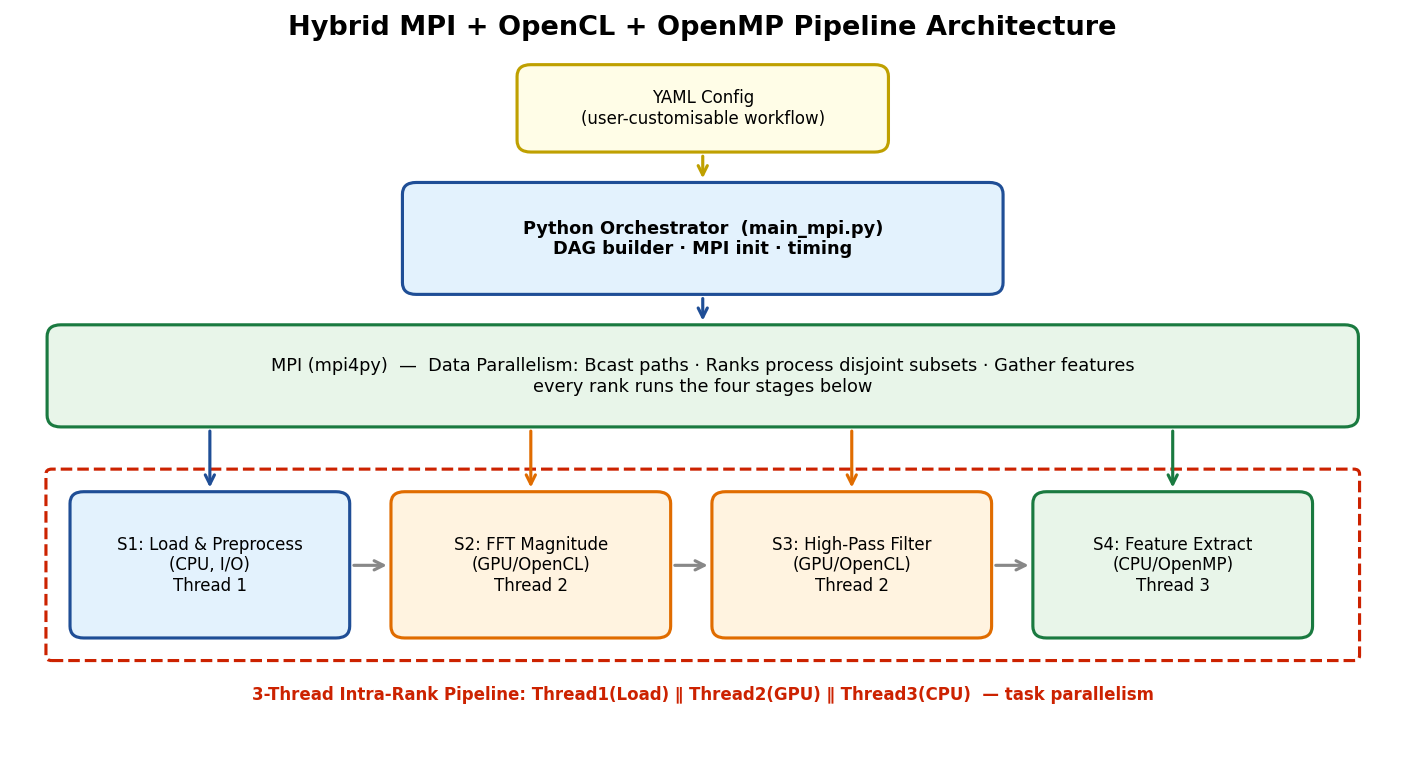
\includegraphics[width=0.85\textwidth]{system_architecture.png}
\caption{System architecture of the hybrid MPI + OpenCL + OpenMP pipeline.}
\label{fig:system-architecture}
\end{figure}

\section{Report Organisation}
\label{sec:organisation}

Chapter~\ref{chap:rationale} states the formal problem and the sequential
baseline. The design then follows Foster's four PCAM steps in order:
partitioning and the task-parallel pipeline in Chapter~\ref{chap:decomp},
communication and agglomeration in Chapter~\ref{chap:comm}, and mapping at the
start of Chapter~\ref{chap:perf}, which then presents the experiments.
Chapter~\ref{chap:conclusions} concludes.
The source code, experiment scripts and raw results are available at
\url{https://github.com/bahatipatrick87/HpcFinalProject}.

\section{Related Work}
\label{sec:related}

\subsection{Parallel FFT Libraries}

FFTW \cite{frigo2005} is a widely used library for computing discrete Fourier
transforms, providing optimised CPU implementations and support for both
shared-memory and distributed-memory execution through its MPI interface
\cite{fftwmpi}. On the GPU side, clFFT \cite{amd2014} provides an OpenCL-based
library for performing fast Fourier transforms on supported GPU platforms.

Unlike these general-purpose libraries, the present project implements a radix-2
two-dimensional FFT directly using OpenCL kernels. This approach provides control
over the GPU computation and its integration with the image-processing pipeline,
while numerical results are validated against a NumPy reference.

\subsection{Hybrid MPI and Accelerator Programming}

Hybrid parallel programming combines distributed-memory communication through MPI
with computation performed by accelerator technologies such as CUDA and OpenCL.
This approach has been studied in applications including stencil computations,
linear algebra, and particle simulations \cite{rauber2013}.

The present project applies this hybrid approach to an end-to-end image-processing
pipeline. MPI distributes image-file workloads across processes, while OpenCL
performs GPU-based FFT and filtering operations and OpenMP parallelises CPU feature
extraction. In addition, a three-thread producer--consumer pipeline overlaps disk
loading, GPU computation, and CPU post-processing.

\subsection{Remote-Sensing Platforms}

Google Earth Engine \cite{gorelick2017} is a cloud-based platform for large-scale
geospatial data processing and analysis. It provides managed access to satellite
imagery and distributed computing capabilities, making it suitable for
remote-sensing applications. However, it offers a different programming model from
the explicit process-level and accelerator-level control used in this project. The
present work focuses on a locally executed, single-node heterogeneous pipeline for
batch processing of remote-sensing images. It combines MPI, OpenCL, and OpenMP to
investigate workload distribution, GPU computation, pipeline overlap, and
communication costs when extracting frequency-domain features from satellite images.

%=======================================================================
\chapter{Problem Rationale}
\label{chap:rationale}
%=======================================================================

\section{Formal Problem Statement}

\begin{quote}\slshape
Given the EuroSAT dataset of Section~\ref{sec:problem},
$\mathcal{D} = \{I_i\}_{i=1}^{N}$ with
$N = 54{,}597$ and each loaded as $I_i \in \mathbb{R}^{64 \times 64 \times 3}$,
design and implement a hybrid parallel pipeline $\Pi$ that performs
frequency-domain filtering and statistical feature extraction on
heterogeneous HPC hardware, minimising total wall-clock time
$T_{\mathrm{total}}$ while maintaining correct results, strong-scaling
efficiency, and runtime reconfigurability.
\end{quote}

\subsection{Mathematical Formulation}

The pipeline $\Pi = (S_1, S_2, S_3, S_4)$ processes each image through
four sequentially dependent stages:

\begin{align}
  I_i' &= \text{Load}(I_i) \in [0,1]^{64\times64\times3}
         \quad\text{(decode and normalise)}, \label{eq:s1}\\
  \hat{I}_i &= \bigl|\mathcal{F}\bigl(I_i'\bigr)\bigr|
         \quad\text{(2D magnitude spectrum)}, \label{eq:s2}\\
  \tilde{I}_i &= \hat{I}_i \circ H
         \quad\text{(element-wise high-pass filter)}, \label{eq:s3}\\
  f_i &= \frac{1}{|\tilde{I}_i|}\sum_{u,v,c}\tilde{I}_i(u,v,c)
         \in\mathbb{R}, \label{eq:s4}
\end{align}

\noindent where Load divides JPEG pixels by 255 and, for GeoTIFFs,
keeps the true-colour bands 4/3/2 and divides the 16-bit reflectance by
2000 (clipped to $[0,1]$); $\mathcal{F}$ denotes the 2D Discrete Fourier Transform
of each channel, $|\cdot|$ the element-wise modulus, and
$\circ$ the element-wise (Hadamard) product. The high-pass mask, applied to
each channel, is
$H(u,v) = 1 - \exp\!\bigl({-d(u,v)^2/50}\bigr)$, where
$u\in\{0,\ldots,W{-}1\}$ and $v\in\{0,\ldots,H_{\mathrm{img}}{-}1\}$ are the
DFT frequency indices with the DC component at $(0,0)$ and no spectrum shift,
and $d(u,v)^2 = \min(u,W{-}u)^2 + \min(v,H_{\mathrm{img}}{-}v)^2$ is the squared
wrap-around distance from DC, for image width $W$ and height $H_{\mathrm{img}}$
(both 64).

\noindent Both the sequential reference
(Section~\ref{sec:seq-baseline}) and the GPU
\texttt{fft\_\discretionary{}{}{}magnitude} kernel compute $|\mathcal{F}|$: the kernel
is a radix-2 Cooley--Tukey FFT applied to the rows and then the columns
of each channel. \texttt{tests\slash{}test\_\discretionary{}{}{}correctness.py} checks it
against \texttt{numpy.fft.fft2}, and
\texttt{experiments\slash{}verify\_\discretionary{}{}{}fft\_\discretionary{}{}{}against\_\discretionary{}{}{}numpy.py}
confirms that the features of all 54{,}597 images agree with a NumPy
computation to within $10^{-6}$ (relative) at $P=1,2,4,8$.

\subsection{Performance Objectives}

The following quantitative objectives guided the design; their measured outcomes
are reported in Chapter~\ref{chap:perf}:
\begin{itemize}
  \item \textbf{Throughput:} exceed 1{,}000 images/s at $P=8$.
  \item \textbf{Communication efficiency:} keep the \texttt{MPI\_Gather} payload
    below 1\,MB.
  \item \textbf{Pipeline overlap:} confirm overlap through per-batch stage timing.
  \item \textbf{Strong scaling:} anticipate sublinear scaling due to shared-resource
    contention (GPU and CPU), analysed in Section~\ref{sec:superlinear-sublinear} and
    quantified using Amdahl's Law \cite{amdahl1967} in Section~\ref{sec:amdahl}.
\end{itemize}

\section{Sequential Baseline}
\label{sec:seq-baseline}

The sequential baseline processes each image completely through all four
stages before advancing to the next (Algorithm~\ref{alg:seq},
Figure~\ref{fig:sequential-flowchart}), where
$M$ is the number of pixels per image, as distinct from the number of
files $N$.
It serves as the reference for the speedups of
Section~\ref{sec:comparative-benchmarking}.

\begin{algorithm}[H]
\caption{Sequential image-processing pipeline.}
\label{alg:seq}
\begin{algorithmic}[1]
\REQUIRE dataset path $\mathcal{P}$
\ENSURE feature vector $\mathbf{v}$, one scalar feature per image
\STATE $\mathcal{L} \leftarrow \textsc{LoadImageList}(\mathcal{P})$
\STATE $\mathbf{v} \leftarrow [\,]$
\FOR{each path $p_i \in \mathcal{L}$}
  \STATE $I_i \leftarrow \textsc{ReadImage}(p_i)$
        \COMMENT{disk I/O, single thread}
  \STATE $I_i' \leftarrow \textsc{Normalise}(I_i)$ \COMMENT{to $[0,1]$, Eq.~\eqref{eq:s1}}
  \STATE $\hat{I}_i \leftarrow |\mathcal{F}(I_i')|$
        \COMMENT{$\mathcal{O}(M\log M)$, CPU}
  \STATE $\tilde{I}_i \leftarrow \hat{I}_i \circ H$
        \COMMENT{$\mathcal{O}(M)$, CPU}
  \STATE $f_i \leftarrow \text{mean}(\tilde{I}_i)$
        \COMMENT{$\mathcal{O}(M)$, CPU}
  \STATE $\mathbf{v}.\text{append}(f_i)$
\ENDFOR
\RETURN $\mathbf{v}$
\end{algorithmic}
\end{algorithm}

\begin{figure}[H]
\centering
\begin{tikzpicture}[
    node distance=0.5cm,
    start/.style={rectangle, rounded corners=4pt, draw=NavyBlue!80,
                  fill=NavyBlue!8, minimum width=3cm, minimum height=0.65cm,
                  font=\small\bfseries, align=center},
    proc/.style={rectangle, draw=DarkSlate, fill=gray!5,
                 minimum width=3.2cm, minimum height=0.65cm,
                 font=\small, align=center},
    io/.style={trapezium, trapezium left angle=68, trapezium right angle=112,
               draw=TealCPU!80, fill=TealCPU!8,
               minimum width=2.8cm, minimum height=0.65cm,
               font=\small, align=center},
    dec/.style={diamond, draw=OrangeGPU!80, fill=OrangeGPU!8,
                aspect=2.5, font=\small, align=center},
    arr/.style={thick,->,>=stealth,DarkSlate}]
  \node (st)   [start]                    {Start};
  \node (init) [proc,  below=of st]       {$\mathbf{v} \leftarrow [\,]$};
  \node (ll)   [io,    below=of init]     {Load image list};
  \node (lp)   [dec,   below=of ll]       {More\\images?};
  \node (rd)   [io,    below=of lp]       {Read image $I_i$};
  \node (nm)   [proc,  below=of rd]       {Normalise $I_i'$ to $[0,1]$};
  \node (ff)   [proc,  below=of nm]       {$\hat{I}_i = |\mathcal{F}(I_i')|$
                                           \quad$\mathcal{O}(M\log M)$};
  \node (fi)   [proc,  below=of ff]       {$\tilde{I}_i = \hat{I}_i \circ H$
                                           \quad$\mathcal{O}(M)$};
  \node (fe)   [proc,  below=of fi]       {$f_i = \text{mean}(\tilde{I}_i)$
                                           \quad$\mathcal{O}(M)$};
  \node (ap)   [proc,  below=of fe]       {Append $f_i$ to $\mathbf{v}$};
  \node (rt)   [proc,  right=3.8cm of lp] {Return $\mathbf{v}$};
  \node (en)   [start, below=of rt]       {End};
  \draw[arr] (st)--(init); \draw[arr](init)--(ll); \draw[arr](ll)--(lp);
  \draw[arr] (lp)--node[left,font=\scriptsize]{Yes}(rd);
  \draw[arr] (rd)--(nm); \draw[arr](nm)--(ff); \draw[arr](ff)--(fi);
  \draw[arr] (fi)--(fe); \draw[arr](fe)--(ap);
  \draw[arr] (ap)--++(-3.2,0)|-(lp);
  \draw[arr] (lp)--node[above,font=\scriptsize]{No}(rt);
  \draw[arr] (rt)--(en);
  \node[right=3pt of ff, text width=2.2cm, font=\scriptsize, color=gray]
       {26.2\,\% of time};
  \node[right=3pt of rd, text width=2.2cm, font=\scriptsize, color=gray]
       {69.8\,\% of time, with normalise};
  \node[right=3pt of ap, text width=2.2cm, font=\scriptsize, color=AlertRed]
       {Serial, no parallelism};
\end{tikzpicture}
\caption{Sequential baseline flowchart.
Each image traverses all four stages before processing begins on the next.
Total time: $T_{\mathrm{seq}} = \sum_{i=1}^{N}
(t_{\mathrm{load}}^{(i)} + t_{\mathrm{FFT}}^{(i)} +
 t_{\mathrm{filt}}^{(i)} + t_{\mathrm{feat}}^{(i)})$.}
\label{fig:sequential-flowchart}
\end{figure}

\subsection{Bottleneck Analysis}

The sequential implementation executes all stages serially and does not use the
GPU or overlap computation. Profiling the full dataset
(\texttt{experiments\slash{}run\_\discretionary{}{}{}sequential\_\discretionary{}{}{}baseline.py},
mean of three trials) gives the following time distribution: loading 69.8\,\%,
FFT 26.2\,\%, filtering 2.9\,\%, and feature extraction 1.2\,\%. Loading and FFT
together account for approximately 96\,\% of execution time, making them the main
optimisation targets. The single-threaded baseline uses only one CPU core and
serves as the reference for evaluating the hybrid implementations.

\section{Background Technologies}
\label{sec:technologies}

MPI \cite{mpiforum2021} provides distributed-memory communication between
processes. OpenCL \cite{stone2010}, a vendor-neutral standard, was chosen over CUDA
for compatibility with the Apple Silicon GPU; Stages~2 and~3 are OpenCL C kernels
embedded in the C++ shared library. OpenMP \cite{openmpARB2018} provides
shared-memory parallelism through compiler directives, applied to Stage~4.

%=======================================================================
\chapter{Decomposition, Partitioning, and Pipeline Design}
\label{chap:decomp}
%=======================================================================

The design follows Foster's PCAM methodology \cite{foster1995}, whose
four steps structure this and the next two chapters:
\textbf{P}artitioning into images and array elements, with the stage DAG
(Sections~\ref{sec:data-decomp}--\ref{sec:task-decomp});
\textbf{C}ommunication (Sections~\ref{sec:interaction}--\ref{sec:aggregation});
\textbf{A}gglomeration into per-rank blocks and 256-image batches
(Section~\ref{sec:agglomeration}); and \textbf{M}apping onto processes,
the GPU and CPU cores (Section~\ref{sec:mapping}). Data parallelism comes
from the partition across ranks (Section~\ref{sec:data-decomp}) and task
parallelism from the three-thread pipeline over the stages
(Section~\ref{sec:prefetch-task-parallelism}).

\section{Data Decomposition: Static Block Distribution}
\label{sec:data-decomp}

The dataset is partitioned across $P$ MPI ranks using a balanced static
block distribution.
Let $Q = \lfloor N/P \rfloor$ and $R = N \bmod P$.
Rank $r \in \{0,\ldots,P{-}1\}$ is assigned images with indices in
$[s_r,\, s_r + n_r)$, where
\begin{equation}
  s_r = rQ + \min(r,R), \qquad
  n_r = \begin{cases}Q+1 & r < R,\\ Q & r \geq R.\end{cases}
  \label{eq:partition}
\end{equation}
For $N = 54{,}597$ and $P = 8$: $Q = 6{,}824$, $R = 5$; ranks
0--4 receive 6{,}825 images and ranks 5--7 receive 6{,}824.

\begin{lstlisting}[language=Python, basicstyle=\ttfamily\footnotesize, columns=flexible,
  caption={MPI data parallelism, simplified from \texttt{dataset\_loader.py} and \texttt{main\_mpi.py}.},
  label=lst:partition]
all_files = comm.bcast(all_files, root=0)  # MPI_Bcast: same list on all ranks
q, r  = len(all_files) // size, len(all_files) % size
start = rank * q + min(rank, r)                    # Eq. (3.1)
end   = start + q + (1 if rank < r else 0)
my_files = all_files[start:end]  # same code, different data (SPMD)
# ... each rank runs S1-S4 on its own my_files, no messages ...
all_lists     = comm.gather(local_list, root=0)     # 1 float/image
all_durations = comm.gather(local_duration, root=0) # T_P = max(.)
\end{lstlisting}

\section{Task Decomposition and Stage Dependency Graph}
\label{sec:task-decomp}

\subsection{Stage Dependency DAG (Single Rank)}

Figure~\ref{fig:task-decomp} is a Directed Acyclic Graph (DAG) whose
nodes are the four pipeline stages and whose directed edges represent
data dependencies.
For one batch on one rank, stages execute strictly left to right.
Node shading encodes the target device (teal = CPU; orange = GPU).

\begin{figure}[H]
\centering
\begin{tikzpicture}[
    node distance=0.9cm and 1.45cm,
    task/.style={rectangle, rounded corners=3pt, draw=DarkSlate, thick,
                 minimum width=2.2cm, minimum height=1.4cm,
                 font=\small, align=center, drop shadow},
    cpu/.style={task, fill=TealCPU!15, draw=TealCPU!60},
    gpu/.style={task, fill=OrangeGPU!15, draw=OrangeGPU!60},
    edge lbl/.style={font=\scriptsize, fill=white, inner sep=1.5pt,
                     midway, above=3pt}
  ]
  \node[cpu] (S1) {$S_1$\\[1pt]\textbf{Load \&}\\\textbf{Preprocess}\\[1pt]{\tiny CPU (I/O)}};
  \node[gpu, right=of S1] (S2) {$S_2$\\[1pt]\textbf{FFT}\\\textbf{Magnitude}\\[1pt]{\tiny GPU (OpenCL)}};
  \node[gpu, right=of S2] (S3) {$S_3$\\[1pt]\textbf{High-Pass}\\\textbf{Filter}\\[1pt]{\tiny GPU (OpenCL)}};
  \node[cpu, right=of S3] (S4) {$S_4$\\[1pt]\textbf{Feature}\\\textbf{Extraction}\\[1pt]{\tiny CPU (OpenMP)}};
  \draw[thick,->,>=stealth] (S1) -- node[edge lbl]{pixels} (S2);
  \draw[thick,->,>=stealth] (S2) -- node[edge lbl]{spectrum} (S3);
  \draw[thick,->,>=stealth] (S3) -- node[edge lbl]{filtered} (S4);
  \begin{scope}[on background layer]
    \node[fit=(S1)(S2)(S3)(S4), inner sep=10pt,
          rectangle, rounded corners=5pt,
          draw=gray!40, fill=gray!4, dashed] {};
  \end{scope}
\end{tikzpicture}
\caption{Stage dependency DAG for one batch on a single MPI rank. Nodes are
stages; edges are data dependencies.}
\label{fig:task-decomp}
\end{figure}

\subsection{MPI Data Distribution}

Figure~\ref{fig:mpi-data-parallelism} illustrates how the dataset is
partitioned across $P$ ranks.
There are \textbf{no peer-to-peer MPI messages}. The only MPI operations are
collectives (Chapter~\ref{chap:comm}): \texttt{MPI\_\discretionary{}{}{}Barrier} before timing,
\texttt{MPI\_\discretionary{}{}{}Bcast} of the file list at startup, and two
\texttt{MPI\_\discretionary{}{}{}Gather} calls at the end, for the features and the per-rank
times.

\begin{figure}[H]
\centering
\begin{tikzpicture}[
    font=\small,
    rank/.style={rectangle, draw=NavyBlue!60, thick, rounded corners=3pt,
                 minimum width=2.3cm, minimum height=1.1cm,
                 align=center, fill=NavyBlue!8, drop shadow},
    darr/.style={->,thick,gray!60},
    hdr/.style={rectangle, draw=gray!50, thick, rounded corners=3pt,
                minimum width=11.5cm, minimum height=0.8cm,
                align=center, fill=gray!8}
  ]
  \node[hdr] (ds) {%
    Full dataset $\mathcal{D}$ ($N=54{,}597$ images):
    rank~0 discovers paths and \texttt{MPI\_\discretionary{}{}{}Bcast}s the list.};
  \node[rank, below=0.9cm of ds, xshift=-3.6cm] (r0)
    {\textbf{Rank 0}\\$D_0$ ($n_0$ images)};
  \node[rank, below=0.9cm of ds]                (r1)
    {\textbf{Rank 1}\\$D_1$};
  \node[rank, below=0.9cm of ds, xshift=3.6cm]  (rp)
    {\textbf{Rank $P{-}1$}\\$D_{P-1}$};
  \node[font=\Large] (dt) at ($(r1)!0.5!(rp)$) {$\cdots$};
  \draw[darr] (ds.south) -- (r0.north);
  \draw[darr] (ds.south) -- (r1.north);
  \draw[darr] (ds.south) -- (rp.north);
\end{tikzpicture}
\caption{MPI data parallelism: the full dataset is broadcast and each
rank retains a contiguous block of paths (Equation~\eqref{eq:partition}), with
$D_0 \cup \cdots \cup D_{P-1} = \mathcal{D}$ and the blocks disjoint. Arrows show
partition ownership, not a processing pipeline between ranks.}
\label{fig:mpi-data-parallelism}
\end{figure}

\subsection{Per-Rank Stage Chain}

Figure~\ref{fig:per-rank-stage-chain} confirms that every rank runs the
same four-stage chain on its local data.
This is replicated-pipeline data parallelism, not rank specialisation
(where different ranks would handle different stages).

\begin{figure}[H]
\centering
\begin{tikzpicture}[
    st/.style={rectangle, draw=DarkSlate, thick, rounded corners=3pt,
               minimum height=0.9cm, minimum width=2.2cm,
               font=\footnotesize, align=center},
    cpu/.style={st, fill=TealCPU!12, draw=TealCPU!50},
    gpu/.style={st, fill=OrangeGPU!12, draw=OrangeGPU!50},
    arr/.style={->,>=stealth,thick},
    node distance=0.9cm and 0.8cm
  ]
  \node[cpu] (s1) {$S_1$: Load\\\scriptsize (CPU)};
  \node[gpu, right=of s1] (s2) {$S_2$: FFT\\\scriptsize (GPU)};
  \node[gpu, right=of s2] (s3) {$S_3$: Filter\\\scriptsize (GPU)};
  \node[cpu, right=of s3] (s4) {$S_4$: Feature\\\scriptsize (CPU/OMP)};
  \draw[arr](s1)--(s2); \draw[arr](s2)--(s3); \draw[arr](s3)--(s4);
\end{tikzpicture}
\caption{Per-rank stage chain: every rank applies the same four stages to each
batch of its own subset, which is data parallelism. Edges are intra-rank data
dependencies; there is no inter-rank compute flow.}
\label{fig:per-rank-stage-chain}
\end{figure}

\section{Task Parallelism: Three-Thread Intra-Rank Pipeline}
\label{sec:prefetch-task-parallelism}

Task parallelism is implemented as a three-thread queue pipeline inside each
rank.

\subsection{Sequential vs.\ Pipeline Execution}

\paragraph{Sequential mode (\texttt{task\_\discretionary{}{}{}parallel\_\discretionary{}{}{}prefetch: false}).}
Each rank loads its full subset, runs FFT and filter on it, then extracts
features, so stages do not overlap. This mode exists for comparison.

\paragraph{Pipeline mode (\texttt{task\_\discretionary{}{}{}parallel\_\discretionary{}{}{}prefetch: true}, default).}
Images are processed in chunks of size \texttt{io\_\discretionary{}{}{}batch\_\discretionary{}{}{}size}, and three
threads per rank form a bounded producer--consumer queue (Listing~\ref{lst:pipeline}):
Thread~1 loads and normalises batch $k{+}1$, Thread~2 applies the two OpenCL kernels
to batch $k$, and Thread~3 runs the OpenMP feature reduction on batch $k{-}1$. These
different operations overlap in wall-clock time on different batches, which is
pipeline/task parallelism. Bounded queues provide back-pressure, a sentinel
propagates shutdown, and the threads overlap because the GIL is released during
disk I/O and every \texttt{ctypes} call.

\noindent\begin{minipage}{\linewidth}
\begin{lstlisting}[language=Python, basicstyle=\ttfamily\footnotesize, columns=flexible,
  caption={Three-thread task-parallel pipeline, simplified from \texttt{batched\_pipeline.py}.},
  label=lst:pipeline]
q1, q2 = queue.Queue(maxsize=3), queue.Queue(maxsize=3)  # bounded queues
def io_worker():                 # Thread 1: load batch k+1
    for chunk in chunks:
        ctx = context.copy(); ctx["input_data"] = load_chunk(chunk)
        q1.put(ctx)
    q1.put(SENTINEL)
def compute_worker():            # Thread 2: GPU stages on batch k
    while (ctx := q1.get()) is not SENTINEL:
        fft_frequency_stage(ctx) # OpenCL fft_magnitude
        filter_stage(ctx)        # OpenCL highpass_filter
        q2.put(ctx)
    q2.put(SENTINEL)
def feature_worker():            # Thread 3: OpenMP features, batch k-1
    while (ctx := q2.get()) is not SENTINEL:
        feature_extraction_stage(ctx)
        all_features.append(ctx["features"])
for t in (t1, t2, t3): t.start() # all three stages run concurrently
for t in (t1, t2, t3): t.join()
\end{lstlisting}
\end{minipage}

\paragraph{Design choice.} An alternative is to express the stages as
OpenMP tasks with asynchronous OpenCL events inside the C++ library.
Python threads with bounded queues were chosen because loading runs in
Python (Pillow, \texttt{tifffile}) and the stages are configured and
orchestrated there: each thread makes blocking calls, yet the stages overlap on
successive batches, and the queues bound memory use.

\subsection{Why Intra-Rank Threads Rather Than Dedicated MPI Ranks}

An inter-rank stage pipeline, in which rank~0 only loads data and passes it to
rank~1 for the FFT, is a valid textbook design. The intra-rank pipeline is preferred
because such a design would send about 12.6\,MB per batch and stage as MPI messages,
where the present design gathers one float per image; because a rank specialised
to the FFT would still contend for the same single GPU; and because images are
independent items suited to MPI distribution, while threads suit overlapping stages
within one rank's batch stream.

\subsection{Gantt Diagram and Timing Evidence}

Figure~\ref{fig:prefetch-pipeline} shows the schedule of the three threads;
Table~\ref{tab:pipeline-timing} gives the measured stage times.

\begin{figure}[H]
\centering
\resizebox{\ifdim\width>\linewidth\linewidth\else\width\fi}{!}{%
\begin{tikzpicture}[
    x=0.083\linewidth, y=1.05cm, font=\footnotesize,
    bar/.style={rectangle, draw=DarkSlate, thick,
                minimum height=0.72cm, align=center, font=\scriptsize},
    io/.style={bar, fill=NavyBlue!14},
    gpub/.style={bar, fill=OrangeGPU!20},
    cpub/.style={bar, fill=TealCPU!16}]
  \draw[->,thick,DarkSlate] (-0.4,-0.6) -- (8.7,-0.6)
    node[right,font=\small]{Wall-clock time $\longrightarrow$};
  \draw[thick,DarkSlate] (-0.4,-0.6) -- (-0.4,2.1);
  \node[left=2pt,font=\small,align=right] at (-0.4, 1.6) {Thread 1 (I/O)};
  \node[left=2pt,font=\small,align=right] at (-0.4, 0.7) {Thread 2 (GPU)};
  \node[left=2pt,font=\small,align=right] at (-0.4,-0.2) {Thread 3 (CPU)};
  % I/O bars
  \node[io,  minimum width=2.1cm] at (1.35, 1.6) {Load $k$};
  \node[io,  minimum width=2.1cm] at (3.75, 1.6) {Load $k{+}1$};
  \node[io,  minimum width=2.1cm] at (6.15, 1.6) {Load $k{+}2$};
  % GPU bars
  \node[gpub,minimum width=2.1cm] at (3.75, 0.7) {FFT+Filter $k$};
  \node[gpub,minimum width=2.1cm] at (6.15, 0.7) {FFT+Filter $k{+}1$};
  % CPU bars
  \node[cpub,minimum width=2.1cm] at (6.15,-0.2) {Feature $k$};
  % Clock tick lines
  \foreach \x in {2.40, 4.80, 7.20}
    \draw[dashed, gray!55] (\x,-0.6) -- (\x,2.1);
  % Overlap bracket
  \draw[<->,very thick,AlertRed] (4.80,2.15) --
    node[above,font=\scriptsize\bfseries,AlertRed]{All three stages overlap}
    (7.20,2.15);
\end{tikzpicture}}
\caption{\textbf{Task parallelism via pipeline:}
three threads stagger Load (I/O), FFT+Filter (GPU), and Feature (CPU)
across successive batches $k$, $k{+}1$, $k{+}2$.
From the second dashed clock-tick line onwards all three threads are
busy at once, each on a different batch (schematic; bar lengths are not
to scale, measured stage times are in Table~\ref{tab:pipeline-timing}).
Implemented with two bounded \texttt{queue.Queue} objects in
\texttt{src\slash{}pipeline\slash{}batched\_\discretionary{}{}{}pipeline.py}.}
\label{fig:prefetch-pipeline}
\end{figure}

\subsection{Parallelism Taxonomy}
\label{sec:data-vs-task}

Table~\ref{tab:parallelism-summary} classifies the parallelism mechanisms of the
implementation.

\begin{table}[!htb]
\centering
\caption{Classification of parallelism mechanisms in the hybrid pipeline.}
\label{tab:parallelism-summary}
\begin{tabular}{@{}p{3.2cm}p{5.0cm}p{4.0cm}@{}}
\toprule
\textbf{Granularity} & \textbf{Mechanism} & \textbf{Parallelism type} \\
\midrule
Across MPI ranks &
  Same pipeline on disjoint image subsets &
  \textbf{Data parallelism} (primary) \\[3pt]
Across successive batches &
  3-thread queue (I/O $\|$ GPU $\|$ CPU) &
  \textbf{Task / pipeline parallelism} \\[3pt]
Within GPU stages (S2, S3) &
  OpenCL work-items over rows, columns, elements &
  Data parallelism (fine-grained) \\[3pt]
Within CPU stage (S4) &
  OpenMP \texttt{parallel for} reduction &
  Data parallelism (fine-grained) \\[3pt]
Stage-to-device assignment &
  CPU for S1/S4, GPU for S2/S3 &
  \textbf{Functional decomposition} \\
\bottomrule
\end{tabular}
\end{table}

Listing~\ref{lst:fine-data} shows the fine-grained mechanisms: OpenCL work-items
that each transform one row or column, and an OpenMP loop whose threads each write
only their own output slot, so no locking is required.

\noindent\begin{minipage}{\linewidth}
\begin{lstlisting}[language=C, basicstyle=\ttfamily\footnotesize, columns=flexible,
  caption={Fine-grained data parallelism on the GPU (OpenCL) and CPU
           (OpenMP), simplified from
           \texttt{src\slash{}pipeline\_\discretionary{}{}{}kernels.cpp}.},
  label=lst:fine-data]
/* S2 on GPU: 2D FFT in two passes; one work-item per row, then per column */
__kernel void fft_magnitude(__global const float* in, __global float* scratch,
                            __global float* out, int width, int height,
                            int channels, int pass) {
    float re[MAX_FFT_LEN], im[MAX_FFT_LEN];
    int gid = get_global_id(0), len = (pass == 0) ? height : width;
    int line = gid % len, c = (gid / len) % channels;
    /* pass 0: real row of `in` -> fft_1d -> complex row of `scratch`
       pass 1: complex column of `scratch` -> fft_1d -> out = sqrt(re^2 + im^2) */
}
/* S4 on CPU: images of one batch split across OpenMP threads */
#pragma omp parallel for schedule(static)
for (int i = 0; i < batch_size; ++i) {
    const float *row = processed_data + (size_t)i * ppi;
    double sum = 0.0;
    for (size_t j = 0; j < ppi; ++j) sum += row[j];
    features_out[i] = (float)(sum / (double)ppi); /* own slot */
}
\end{lstlisting}
\end{minipage}

Figure~\ref{fig:parallel-patterns} contrasts the two patterns: only (B), in which
distinct operations overlap in time on different data, is task parallelism; (A)
alone, however many ranks are used, remains data parallelism.

\begin{figure}[H]
\centering
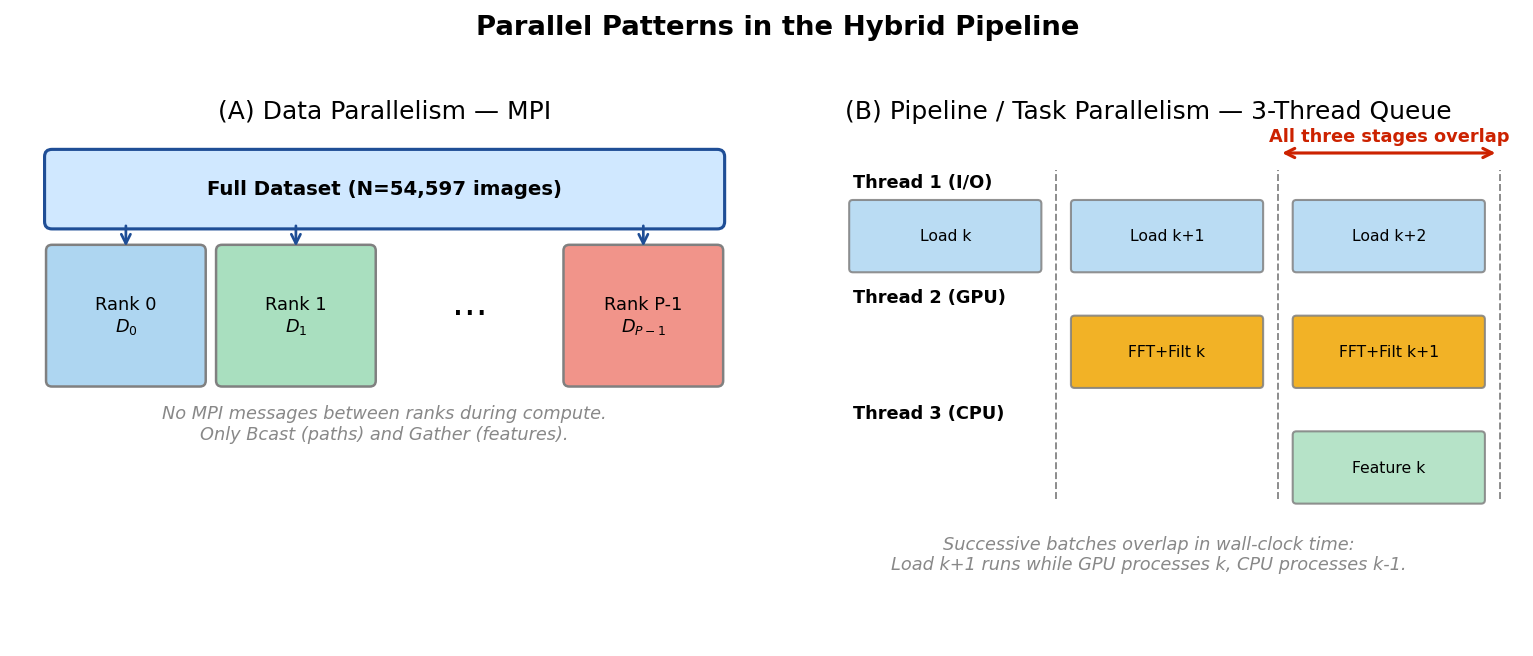
\includegraphics[width=0.9\textwidth]{parallel_patterns.png}
\caption{The two parallelism patterns of the hybrid pipeline: (A) MPI data
parallelism across ranks, and (B) three-thread task parallelism across successive
batches within one rank.}
\label{fig:parallel-patterns}
\end{figure}

\section{User-Customisable Workflow}
\label{sec:user-workflow}

A YAML-driven Directed Acyclic Graph (DAG) engine
(\texttt{src\slash{}pipeline\slash{}task\_\discretionary{}{}{}graph.py}) allows users to
reconfigure the pipeline at runtime without recompilation. Stages declare the data
they read and write (pixels, spectrum, filtered, features); dependencies between
these stages are validated on every rank using Kahn's topological sort before
processing begins. Users can enable, disable, or reorder stages in
\texttt{config\slash{}pipeline.yaml}. Missing inputs or unknown stage names cause a
configuration error, while unused outputs generate a warning. The three-thread
pipeline requires the default stage order; other valid stage orders use the
sequential DAG scheduler. Listing~\ref{lst:yaml} shows the main configuration
options, and Figure~\ref{fig:dag-model} illustrates the execution model.

\noindent\begin{minipage}{\linewidth}
\begin{lstlisting}[basicstyle=\ttfamily\footnotesize, columns=flexible, caption={Workflow configuration (excerpt of \texttt{config\slash{}pipeline.yaml}).}, label=lst:yaml]
dataset:
  root: "data/EuroSAT"
  target_width: 64
  target_height: 64
pipeline:
  channels: 3
  stages:
    - io
    - fft
    - filter
    - feature
  task_parallel_prefetch: true
  io_batch_size: 256
\end{lstlisting}
\end{minipage}

\begin{figure}[H]
\centering
\resizebox{\ifdim\width>\linewidth\linewidth\else\width\fi}{!}{%
\begin{tikzpicture}[
    node distance=0.55cm,
    stg/.style={rectangle, rounded corners=3pt, minimum width=4.6cm,
                minimum height=0.9cm, draw=DarkSlate, thick,
                font=\small, align=center, drop shadow},
    io/.style={stg, fill=TealCPU!12,   draw=TealCPU!55},
    gp/.style={stg, fill=OrangeGPU!12, draw=OrangeGPU!55},
    arr/.style={thick,->,>=stealth},
    edgelbl/.style={font=\scriptsize, fill=white, inner sep=1.5pt,
                     midway, right=1pt}
  ]
  \node[io] (s1) {$S_1$: Load \& Preprocess\\{\scriptsize CPU (I/O)}};
  \node[gp, below=of s1] (s2) {$S_2$: FFT Magnitude\\{\scriptsize GPU (OpenCL)}};
  \node[gp, below=of s2] (s3) {$S_3$: High-Pass Filter\\{\scriptsize GPU (OpenCL)}};
  \node[io, below=of s3] (s4) {$S_4$: Feature Extraction\\{\scriptsize CPU (OpenMP)}};
  \draw[arr] (s1) -- node[edgelbl]{pixels}   (s2);
  \draw[arr] (s2) -- node[edgelbl]{spectrum} (s3);
  \draw[arr] (s3) -- node[edgelbl]{filtered} (s4);
  \begin{scope}[on background layer]
    \node[fit=(s1)(s2)(s3)(s4), inner sep=10pt,
          rectangle, rounded corners=5pt,
          draw=gray!40, fill=gray!4, dashed] {};
  \end{scope}
  \node[rectangle, draw=gray!50, dashed, fill=yellow!6,
        at={($(s2.east)!0.5!(s3.east)+(3.4,0)$)},
        text width=3.6cm, font=\ttfamily\scriptsize, align=left,
        label={[font=\scriptsize\itshape,text=gray!70]above:runtime
          \texttt{stages} list}] (yaml){
    stages:\\
    \space\space- io\\
    \space\space- fft\\
    \space\space- filter\\
    \space\space- feature
  };
  \draw[-stealth, thick, gray!60, dashed] (yaml.north west) -- (s1.east);
  \draw[-stealth, thick, gray!60, dashed] (yaml.south west) -- (s4.east);
\end{tikzpicture}}
\caption{DAG execution model. Each node is a stage constructed at
runtime; edges carry the data passed between stages (teal = CPU,
orange = GPU). Reordering or removing entries in the YAML \texttt{stages}
list (inset) rebuilds and re-validates the DAG without recompilation.}
\label{fig:dag-model}
\end{figure}

%=======================================================================
\chapter{Communication, Aggregation, and Agglomeration}
\label{chap:comm}
%=======================================================================

This chapter covers the second and third PCAM steps: communication, including the
aggregation of results, and agglomeration.

\section{Interaction Graph and Communication Costs}
\label{sec:interaction}

Figure~\ref{fig:interaction} shows the communicating entities and
Table~\ref{tab:comm-costs} the volume and cost of each communication.

\begin{figure}[H]
\centering
\begin{tikzpicture}[
    x=0.92cm, y=0.92cm, font=\footnotesize, >=stealth,
    rank/.style={rectangle, draw=NavyBlue!50, thick, fill=NavyBlue!8,
                 minimum width=1.7cm, minimum height=0.88cm,
                 font=\scriptsize, align=center, rounded corners=3pt},
    gpun/.style={rectangle, draw=OrangeGPU!60, thick, fill=OrangeGPU!10,
                 minimum width=3.0cm, minimum height=0.88cm,
                 align=center, rounded corners=3pt},
    diskn/.style={rectangle, draw=gray!60, thick, fill=gray!8,
                  minimum width=3.2cm, minimum height=0.72cm,
                  align=center, rounded corners=3pt},
    mpi/.style={->,thick,NavyBlue!70},
    io/.style={ ->,thick,OrangeGPU!60,dashed}
  ]
  \node[diskn, minimum width=10.3cm] (dk) at (4.35,5.5) {Storage (image files)};
  \node[rank] (r0) at (0.0,2.6) {Rank 0\\(root)};
  \node[rank] (r1) at (2.9,2.6) {Rank 1};
  \node[rank] (r2) at (5.8,2.6) {Rank 2};
  \node[rank] (r3) at (8.7,2.6) {Rank $P{-}1$};
  \node[gpun, minimum width=10.3cm] (gpu) at (4.35,-0.4)
    {Shared GPU (OpenCL) --- 1 device; all ranks contend};
  % disk reads and host--device transfers: straight, one per rank
  \foreach \x/\r in {-0.4/r0, 2.5/r1, 5.4/r2, 8.3/r3}{
    \draw[io] (\x,5.5-0.39) -- (\x,3.08);
    \draw[<->,thick,OrangeGPU!60,dashed] (\x,2.12) -- (\x,0.08);
  }
  % MPI_Bcast: rank 0 to every other rank
  \draw[thick,NavyBlue!70] (0.4,3.08) -- (0.4,3.8) -- (9.1,3.8);
  \foreach \x in {3.3,6.2,9.1} \draw[mpi] (\x,3.8) -- (\x,3.08);
  % MPI_Gather: every rank to rank 0
  \draw[thick,NavyBlue!70] (9.1,2.12) -- (9.1,1.1) -- (0.4,1.1);
  \foreach \x in {3.3,6.2} \draw[thick,NavyBlue!70] (\x,2.12) -- (\x,1.1);
  \draw[mpi] (0.4,1.1) -- (0.4,2.12);
  % labels, right of the figure, clear of every line
  \node[right,font=\scriptsize,text=OrangeGPU!90!black,align=left] at (9.75,4.6) {disk reads\\3.05\,GB};
  \node[right,font=\scriptsize,text=NavyBlue!80,align=left] at (9.75,3.65)
    {\texttt{MPI\_Bcast}\\path list, $\approx$5\,MB};
  \node[right,font=\scriptsize,text=NavyBlue!80,align=left] at (9.75,1.35)
    {\texttt{MPI\_Gather}\\1 float/image, \textbf{213\,KB}};
  \node[right,font=\scriptsize,text=OrangeGPU!90!black,align=left] at (9.75,0.55) {H2D/D2H\\$\sim$12.6\,MB/batch};
\end{tikzpicture}

\vspace{0.5em}
\noindent\fcolorbox{gray!40}{white}{%
\begin{minipage}{0.95\linewidth}\footnotesize
  \textbf{Legend.}
  \textcolor{NavyBlue!70}{\textbf{Solid blue}}: MPI collectives
  (\texttt{MPI\_\discretionary{}{}{}Bcast}, \texttt{MPI\_\discretionary{}{}{}Gather}).
  \textcolor{OrangeGPU!80}{\textbf{Orange dashed}}: disk reads and
  OpenCL host--device transfers (H2D/D2H). The timing barrier and the gather of
  per-rank times are not drawn.
\end{minipage}}
\caption{Interaction graph. All MPI ranks share one physical GPU.}
\label{fig:interaction}
\end{figure}

\begin{table}[H]
\centering
\caption{Communication and interaction costs for the full EuroSAT dataset
($N=54{,}597$, $P=8$).}
\label{tab:comm-costs}
\begin{tabular}{@{}p{4.9cm}p{2.7cm}p{2.5cm}c@{}}
\toprule
\textbf{Operation} & \textbf{Type} & \textbf{Volume} &
\textbf{Run-time share} \\
\midrule
Path list \texttt{MPI\_\discretionary{}{}{}Bcast} & MPI collective & $\approx$5\,MB &
  ${<}1\%$ \\[3pt]
Image loading & Disk I/O         & 3.05\,GB read & $\approx$98\% \\[3pt]
GPU-stage dispatch$^{\dagger}$ (H2D + kernel + D2H + API call) & OpenCL & $\sim$12.6\,MB/batch &
  $\approx$12\% \\[3pt]
Feature \texttt{MPI\_\discretionary{}{}{}Gather}   & MPI collective & \textbf{213\,KB} &
  ${<}0.1\%$ \\[3pt]
Per-rank time \texttt{MPI\_\discretionary{}{}{}Gather} & MPI collective & 1 float/rank &
  ${<}0.1\%$ \\[3pt]
\texttt{MPI\_\discretionary{}{}{}Barrier} (timing) & MPI collective & 0\,B &
  ${<}0.1\%$ \\
\bottomrule
\end{tabular}
\vspace{2pt}
\footnotesize $^{\dagger}$Run-time shares for image loading and GPU-stage
dispatch are the mean busy times of the GeoTIFF ranks at $P{=}8$ from
Table~\ref{tab:stage-breakdown} ($S_1$ versus $S_2{+}S_3$ combined), as
a fraction of their wall time; the stages overlap, so the shares do not sum to
100\,\%. MPI shares are measured
(\texttt{experiments\slash{}measure\_\discretionary{}{}{}mpi\_\discretionary{}{}{}collectives.py}): about 9\,ms for the
broadcast and under 0.1\,ms for the others, against $T_8 = 5.37$\,s.
\end{table}

\section{Feature Aggregation Strategy}
\label{sec:aggregation}

Gathering raw pixel data after processing would require transferring
$54{,}597 \times 64 \times 64 \times 3 \times 4\,\mathrm{B} = 2.68\,\mathrm{GB}$
over MPI, a serialisation bottleneck at rank~0. Instead, each rank reduces every
image to one scalar (Equation~\eqref{eq:s4}), so the gather carries
$N \times 4\,\mathrm{B} = 213\,\mathrm{KB}$, a reduction of more than $12{,}000\times$.


\section{Agglomeration}
\label{sec:agglomeration}

Agglomeration groups the fine-grained units of work (one image, one array element)
into coarser ones sized to amortise fixed per-unit overheads. Unlike the
\emph{aggregation} of Section~\ref{sec:aggregation}, which combines computed
results, it groups \emph{work} before it is computed. Two decisions are made.

\paragraph{Data agglomeration: contiguous per-rank blocks.}
Each rank's share (Equation~\eqref{eq:partition}) is one contiguous range of the
file list, not a cyclic distribution. This balances image \emph{counts}, not
\emph{cost}: the list, in directory-walk order, holds 14{,}000
JPEGs, then the 27{,}597 GeoTIFFs, which take more than twice as long to
load, then 13{,}000 JPEGs. At $P=2$ each rank gets an even mix, but from
$P=4$ the middle ranks hold mainly GeoTIFFs and finish last
(Section~\ref{sec:stage-breakdown}).

\paragraph{Task agglomeration: fixed-size batches.}
Within each rank, images are grouped into batches of
\texttt{io\_\discretionary{}{}{}batch\_\discretionary{}{}{}size} images (default 256), which trades off two costs:
\begin{itemize}[noitemsep]
  \item \textbf{Larger batches} amortise the fixed cost of each GPU
    dispatch (Section~\ref{sec:gpu-idle-check}). A batch size of 256 gives 214 dispatches per stage at $P=1$ and
    216 in total at $P=8$ (27 per rank), against 854 and 856 at a batch size of
    64; each FFT dispatch runs its two passes.
  \item \textbf{Smaller batches} limit in-flight memory. A batch is $\approx$12.6\,MB of pixels, and
    $\approx$38\,MB once it carries its spectrum and filtered arrays. An
    approximate upper bound on the image data in flight per rank is therefore
    $\approx$240\,MB: both \texttt{queue.Queue(maxsize=3)} queues full (3 batches
    of 12.6\,MB and 3 of 38\,MB) plus one batch held by each of the three worker
    threads. This estimate excludes the interpreter, the libraries and the FFT's
    temporary buffers; a $P=1$ run's measured peak resident memory, interpreter
    included, is 116--153\,MB.
\end{itemize}
The value 256 is a middle ground between the two, not exhaustively tuned.
Table~\ref{tab:agglomeration-mapping} summarises these decisions.

\begin{table}[H]
\centering
\caption{Agglomeration and mapping summary. Rows 1--2 are the
agglomeration decisions above; rows 3--5 anticipate the fourth PCAM
step, the mapping of Section~\ref{sec:mapping}.}
\label{tab:agglomeration-mapping}
\begin{tabular}{@{}p{2.9cm}p{3.6cm}p{4.3cm}p{2.3cm}@{}}
\toprule
\textbf{Decision} & \textbf{Strategy chosen} & \textbf{Rationale} &
\textbf{Granularity} \\
\midrule
Data agglomeration (per rank) &
  Contiguous block (Eq.~\eqref{eq:partition}) &
  Equal image counts; simplest closed-form split; same images per rank
  on every run (JPEG/GeoTIFF cost differs, \S\ref{sec:stage-breakdown}) &
  $\approx$6,825 img/rank at $P{=}8$ \\[4pt]
Task agglomeration (per batch) &
  Fixed batch, \texttt{io\_\discretionary{}{}{}batch\_\discretionary{}{}{}size} &
  Amortises the fixed GPU dispatch cost (\S\ref{sec:gpu-idle-check}) vs.\
  pipeline latency/memory &
  256 img/batch ($\approx$12.6\,MB) \\[4pt]
Mapping: ranks $\to$ processes &
  1 MPI rank = 1 OS process &
  Standard MPI execution model &
  $P\in\{1,2,4,8\}$ measured \\[4pt]
Mapping: ranks $\to$ GPU &
  \texttt{device\_\discretionary{}{}{}idx = rank \% num\_\discretionary{}{}{}devices} &
  Shares the one available GPU here; multi-GPU needs no code change &
  1 shared GPU (this testbed) \\[4pt]
Mapping: OpenMP $\to$ cores &
  \texttt{\#pragma omp parallel for} in Stage~4 &
  OS-scheduled across available CPU cores &
  Up to 10 cores (4P\,+\,6E) \\
\bottomrule
\end{tabular}
\end{table}

%=======================================================================
\chapter{Performance Evaluation}
\label{chap:perf}
%=======================================================================

\section{Testbed and Hardware Mapping}
\label{sec:mapping}

This section completes the design with the fourth PCAM step, mapping, and describes
the hardware on which the experiments run.

\subsection{Testbed Hardware}

\begin{itemize}[noitemsep]
  \item \textbf{Machine:} MacBook Air 13-inch, M4, 2025 (fanless laptop;
    model identifier Mac16,12, model number MC6T4T/A).
  \item \textbf{Processor:} Apple M4 (ARM64; 4 performance
    cores + 6 efficiency cores, 10 cores total).
  \item \textbf{GPU:} \textbf{1 integrated 8-core GPU} (unified memory architecture; no discrete PCIe
    GPU).
  \item \textbf{Memory:} 16\,GB Unified RAM
    (120\,GB/s bandwidth: manufacturer specification \cite{applem4},
    not measured here).
  \item \textbf{Storage:} 256\,GB Apple NVMe SSD (AP0256Z).
  \item \textbf{Software:} macOS~26.6.2, Open~MPI~5.0.8,
    mpi4py~4.1.1, Python~3.12.12, Apple Clang~21.
\end{itemize}

This SoC has one physical GPU, so GPU count cannot be varied here. The runtime
selects devices round-robin
(\texttt{device\_\discretionary{}{}{}idx = mpi\_\discretionary{}{}{}rank \% num\_\discretionary{}{}{}devices}), so a
multi-GPU node needs no code change; Section~\ref{sec:gpu-scaling} instead
sweeps concurrent demand on the one GPU.

\subsection{Hierarchical Mapping Strategy}

The mapping of software entities to hardware resources follows a four-level
hierarchy, illustrated in Figure~\ref{fig:mapping}.
\begin{enumerate}
  \item \textbf{MPI ranks $\rightarrow$ OS processes.} Each MPI rank is an
    independent OS process scheduled onto available CPU cores by macOS. The
    operating system does not guarantee hard CPU-core pinning, so this is
    scheduling rather than fixed assignment. Core type matters: a process confined
    to the efficiency cores (\texttt{taskpolicy -c background}) was measured to
    decode images about 3$\times$ more slowly (Section~\ref{sec:superlinear-sublinear}).
  \item \textbf{MPI ranks $\rightarrow$ OpenCL command queues.} Each rank creates a
    private OpenCL command queue on the shared GPU through
    \texttt{init\_\discretionary{}{}{}opencl(rank)}. All ranks share the same physical GPU.
  \item \textbf{OpenMP threads $\rightarrow$ CPU cores.} Stage~4 distributes its
    per-image mean reduction across CPU cores using \texttt{\#pragma omp parallel for}.
  \item \textbf{OpenCL work-items $\rightarrow$ GPU execution.} Stages~2 and~3
    launch GPU work-items that run in parallel: one per row and then per column of
    each channel in Stage~2 (Listing~\ref{lst:fine-data}), and one per array
    element in Stage~3.
\end{enumerate}

\begin{figure}[H]
\centering
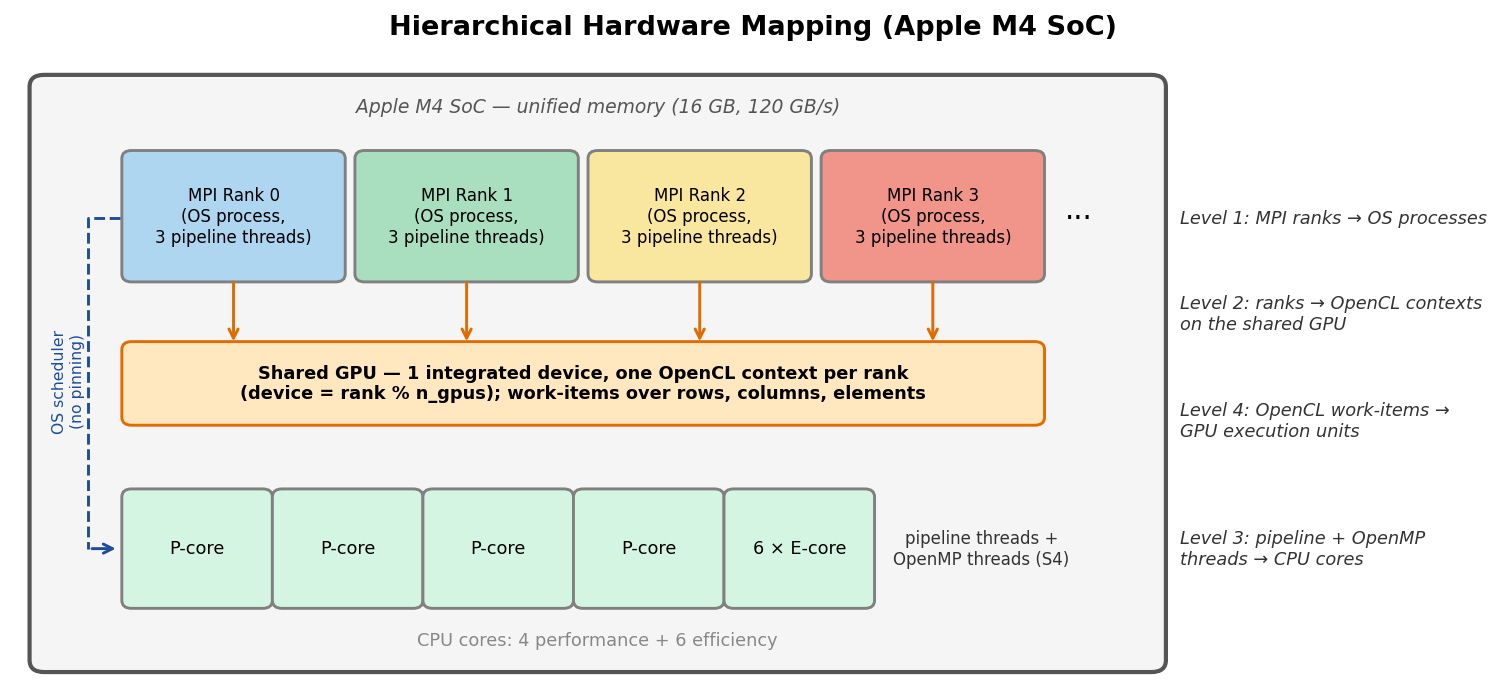
\includegraphics[width=0.85\textwidth]{mapping_hierarchy.png}
\caption{Hierarchical mapping of software entities to hardware resources.}
\label{fig:mapping}
\end{figure}

\section{Experimental Methodology}
\label{sec:methodology}

Each rank's wall-clock time runs from a barrier after OpenCL initialisation to the
end of its local pipeline, and scaling tables use the maximum across ranks. Unless
stated otherwise, experiments use the three-thread pipeline. Each timed run follows
an untimed run of the same configuration, and values are averages of repeated runs
interleaved across configurations.

\subsection{File-Cache State and Experimental Repeatability}

Execution times depend strongly on the operating system's file cache. When the
3.05\,GB dataset is mostly cached, a $P=1$ run takes approximately 6.3\,s. When
images must be read from disk, the run takes approximately 16\,s and involves around
3\,GB of disk reads. Most full-dataset experiments therefore used a 7\,GB
memory-holding process (\texttt{experiments\slash{}hold\_\discretionary{}{}{}memory.py}) to
encourage disk-based reading. However, monitoring with \texttt{iostat} showed that
not all experiments ran under identical cache conditions: strong scaling, the
sequential comparison, the stage breakdown, the partition comparison and GPU
concurrency at $P=8$ were predominantly disk-based, while weak scaling and the other
smaller experiments were mostly cached. The stage-overlap timing and the pipeline
on/off comparison ran without held memory (Section~\ref{sec:pipeline-payoff}). GPU-stage timing and the OpenMP FFT sweep did not
involve dataset file access.

Repeat sessions reproduced the main qualitative findings, but absolute execution
times varied with cache state. For example, a session whose first run measured
$T_1 = 11.9$\,s fell to 6.3\,s as held memory was swapped out and the dataset
became cached; this session was discarded. A subsequent session with 9\,GB of
actively held memory (\texttt{hold\_memory.py 9 -{}-active}, 5 rounds) was more
stable, giving $T_1 = 13.05$\,s, $T_8 = 5.96$\,s, $S_2 = 1.77$, $S_4 = 2.01$ and
$S_8 = 2.19$. With the dataset cached (3 rounds), $T_1 = 6.80$\,s, $T_8 = 2.64$\,s,
$S_2 = 1.79$, $S_4 = 2.03$ and $S_8 = 2.58$
(\texttt{results\slash{}reproduction\_\discretionary{}{}{}20261103/}).
Across the reported sessions, the measured $S_8$ ranged from approximately 2.2 to
3.2, so absolute timings must be read with their cache state. Nevertheless, the main findings remained consistent: image loading
was the major bottleneck, load imbalance appeared from $P=4$, the OpenMP pipeline
sweep showed little improvement, and cyclic partitioning improved performance.

\section{Strong Scaling}
\label{sec:strong-scaling}

\subsection{Superlinear vs.\ Sublinear Speedup}
\label{sec:superlinear-sublinear}

Three mechanisms can in principle produce speedup above the ideal $S_P = P$: smaller
per-rank working sets that fit in cache, better GPU occupancy when several ranks
share it, and measurement artefacts that inflate $T_1$. None is observed:
Table~\ref{tab:strong-scaling} shows $S_8 \approx 3.17$, and the speedup is sublinear
from $P = 2$ onwards.

At $P=2$ scaling is near-linear ($S_2 = 1.86$, efficiency 92.9\,\%),
because each rank receives an even mix of JPEGs and GeoTIFFs, so the two
ranks finish close together (8.19\,s and 9.17\,s). From $P=4$ the dominant
limit is load imbalance: the contiguous partition
(Section~\ref{sec:agglomeration}) gives the outer ranks mainly JPEGs and
the middle ranks mainly GeoTIFFs, whose Load stage takes more than twice
as long. The ``Fastest rank'' column of Table~\ref{tab:strong-scaling}
shows the JPEG ranks finishing at about half of $T_P$ or earlier and then waiting.
Section~\ref{sec:stage-breakdown} isolates the effect. The secondary
effect is the shared GPU: all ranks submit to one device
(Section~\ref{sec:gpu-idle-check}). The CPU is shared too: eight ranks
of three threads each run on ten cores, only four of them performance
cores.

\subsection{Results}

\begin{table}[H]
\centering
\caption{Strong-scaling results for the full EuroSAT dataset
($N = 54{,}597$ images): average of 5 interleaved rounds (\texttt{results\slash{}strong\_\discretionary{}{}{}scaling.csv}).
Speedup $S_P = T_1/T_P$; efficiency $E_P = S_P/P$; ``Fastest rank'' is
the mean time of the quickest rank, against $T_P$ for the slowest.}
\label{tab:strong-scaling}
\begin{tabular}{@{}crrrrrr@{}}
\toprule
$P$ & \textbf{Images/rank} & $T_P$ [s] & \textbf{Fastest rank} [s] &
$S_P$ & $E_P$ & \textbf{Throughput [img/s]} \\
\midrule
1 & 54,597 & 17.03 & 17.03 & 1.00 & 100.0\% & 3,206 \\
2 & 27,299 &  9.17 &  8.19 & 1.86 &  92.9\% & 5,956 \\
4 & 13,650 &  7.06 &  3.16 & 2.41 &  60.3\% & 7,732 \\
8 &  6,825 &  5.37 &  2.60 & 3.17 &  39.7\% & \textbf{10,170} \\
\bottomrule
\end{tabular}
\end{table}

\begin{figure}[H]
\centering
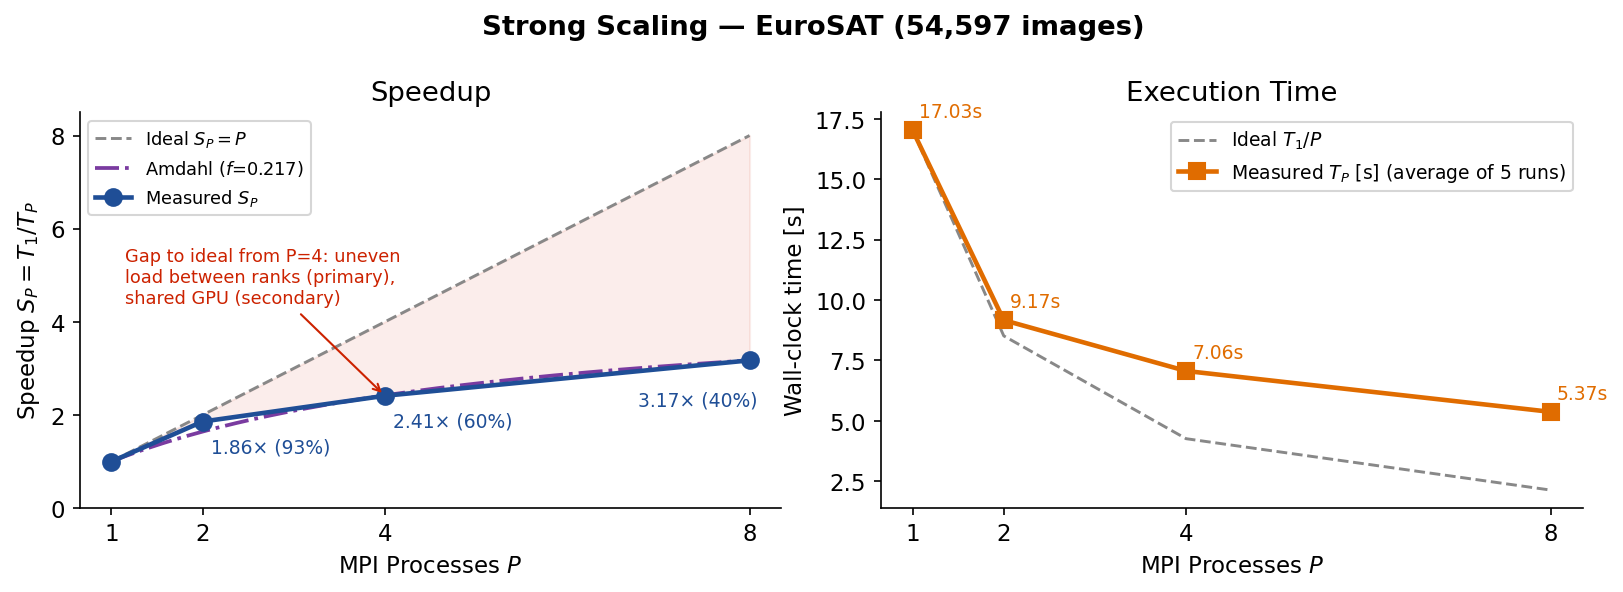
\includegraphics[width=0.92\textwidth]{strong_scaling_optimized.png}
\caption{Strong-scaling speedup against the ideal $S_P = P$ and the Amdahl's Law
fit of Section~\ref{sec:amdahl}.}
\label{fig:strong-scaling}
\end{figure}

\subsection{Theoretical Bound: Amdahl's Law}
\label{sec:amdahl}

Amdahl's Law \cite{amdahl1967} bounds the speedup of a fixed-size problem on $P$
processing elements when a fraction $f$ of the work does not shrink with $P$:
\begin{equation}
  S_P = \frac{1}{f + \dfrac{1-f}{P}},
  \qquad\qquad
  S_\infty = \lim_{P \to \infty} S_P = \frac{1}{f}.
  \label{eq:amdahl}
\end{equation}

Solving Equation~\eqref{eq:amdahl} for $f$ using the $P=8$ measurement
in Table~\ref{tab:strong-scaling} ($S_8 = 3.17$) gives
\[
  f = \frac{P/S_P - 1}{P - 1}\bigg|_{P=8} \approx 0.217 \quad (22\,\%),
\]
implying a ceiling of $S_\infty = 1/f \approx 4.6\times$ on this testbed with the
current partitioning, untested since the testbed never ran $P>8$. Because $f$ is
fitted from one point, moving it by 0.06 either way gives ceilings of $6.35\times$ and
$3.60\times$
(Figure~\ref{fig:amdahl-sensitivity}).

\begin{table}[H]
\centering
\caption{Measured speedup versus Amdahl's Law, $f=0.217$ fitted at
$P=8$, and the Karp--Flatt metric $e$
(\texttt{experiments\slash{}analyze\_\discretionary{}{}{}amdahl.py}).}
\label{tab:amdahl-fit}
\begin{tabular}{@{}crrrr@{}}
\toprule
$P$ & \textbf{Measured $S_P$} & \textbf{Amdahl $S_P$} &
\textbf{Difference} & \textbf{Karp--Flatt $e$} \\
\midrule
1 & 1.00 & 1.00 & 0.0\,\% & --- \\
2 & 1.86 & 1.64 & $+$13.1\,\% & 0.076 \\
4 & 2.41 & 2.42 & $-$0.4\,\% & 0.220 \\
8 & 3.17 & 3.17 & 0.0\,\% (fit point) & 0.217 \\
\bottomrule
\end{tabular}
\end{table}

Table~\ref{tab:amdahl-fit} compares the fit with the measurements. It is within
1\,\% at $P=4$ and exact at $P=8$ by construction, but
underestimates the speedup at $P=2$ by 13.1\,\%, where the ranks are balanced and the
load imbalance that dominates $f$ has not yet appeared. $f$ is therefore not a literal
serial-code fraction but an effective non-scaling fraction, dependent on $P$.

\paragraph{Karp--Flatt metric.} The experimentally determined serial fraction
\cite{karp1990}, $e = (1/S_P - 1/P)/(1 - 1/P)$, tests whether $f$ really is
constant. At $P=8$ it equals the fitted $f$ by construction. It rises from
0.076 at $P=2$ to 0.220 at $P=4$ and then stays flat at 0.217: the non-scaling
fraction is not a fixed serial part of the code but appears when the load
imbalance does. In the repeat session of Section~\ref{sec:methodology} the fit gave
$f = 0.38$ and a ceiling of $2.6\times$, with $e$ of 0.128, 0.330 and 0.379: the same
pattern, at a different level. The ceiling is therefore not a fixed property of
the code. The symbol $f$ alone denotes this fraction; $f_i$ in
Chapter~\ref{chap:rationale} is a per-image feature.

\begin{figure}[H]
\centering
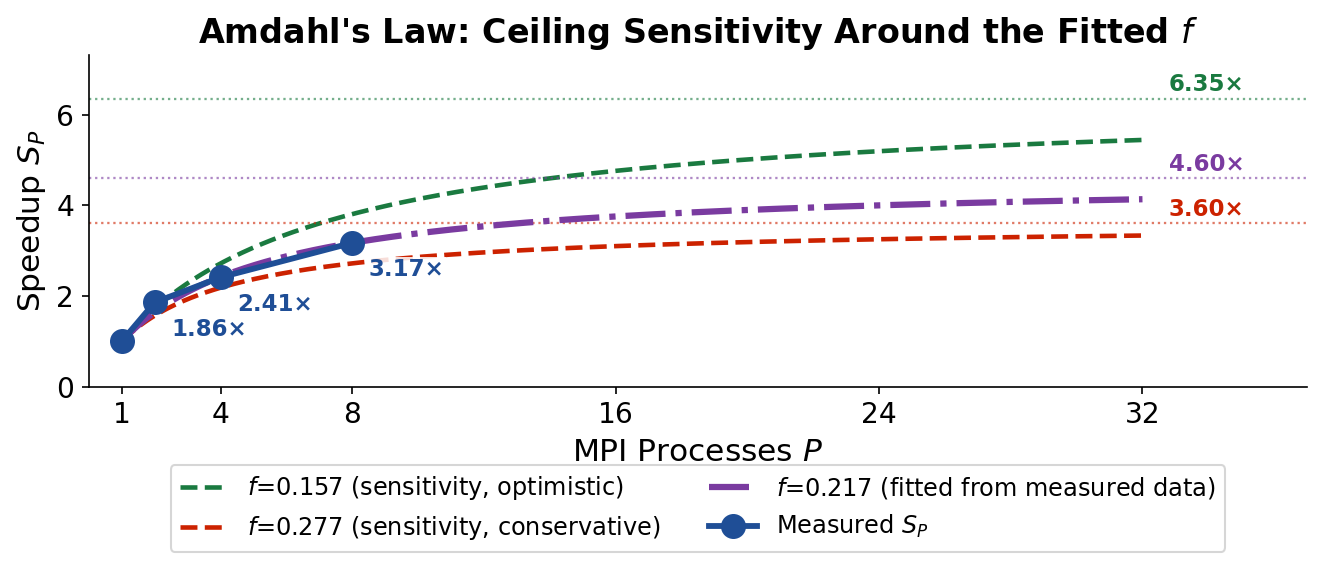
\includegraphics[width=0.78\textwidth]{amdahl_sensitivity.png}
\caption{Sensitivity of the Amdahl's Law ceiling to the fitted effective non-scaling
fraction. The thick curve ($f=0.217$) is the fit of Figure~\ref{fig:strong-scaling};
the dashed curves ($f=0.157$, $f=0.277$) are hypothetical, and all curves beyond
$P=8$ are projections.}
\label{fig:amdahl-sensitivity}
\end{figure}

\section{Weak Scaling}
\label{sec:weak-scaling}

Weak scaling holds the workload at 1{,}000 images per rank. Rank $r$ processes files
$[1000r, 1000(r{+}1))$, all JPEGs for $P \le 8$, and efficiency is
$E_P^{\mathrm{weak}} = T_1/T_P$. Table~\ref{tab:weak-scaling} and
Figure~\ref{fig:weak-scaling} give the results.

\begin{table}[H]
\centering
\caption{Weak-scaling results (1{,}000 images per rank): 4 interleaved
rounds, averages; raw data in
\texttt{results\slash{}weak\_\discretionary{}{}{}scaling\_\discretionary{}{}{}raw\_\discretionary{}{}{}trials.csv}.}
\label{tab:weak-scaling}
\begin{tabular}{@{}crrrr@{}}
\toprule
$P$ & \textbf{Total images} & $T_P$ [s] & $T_P/T_1$ &
$E_P^{\mathrm{weak}}$ \\
\midrule
1 & 1,000 & 0.180 & 1.00 &  100.0\% \\
2 & 2,000 & 0.188 & 1.05 &   95.5\% \\
4 & 4,000 & 0.258 & 1.43 &   69.7\% \\
8 & 8,000 & 0.383 & 2.13 &   46.9\% \\
\bottomrule
\end{tabular}
\end{table}

Efficiency declines from $95.5\,\%$ at $P=2$ to $46.9\,\%$ at $P=8$, as growing total work increases demand on the shared CPU cores and GPU. Every rank
processes only JPEGs, so this decline is not the JPEG/GeoTIFF imbalance. The runs
varied by under 9\,\% across the 4 rounds.

\begin{figure}[H]
\centering
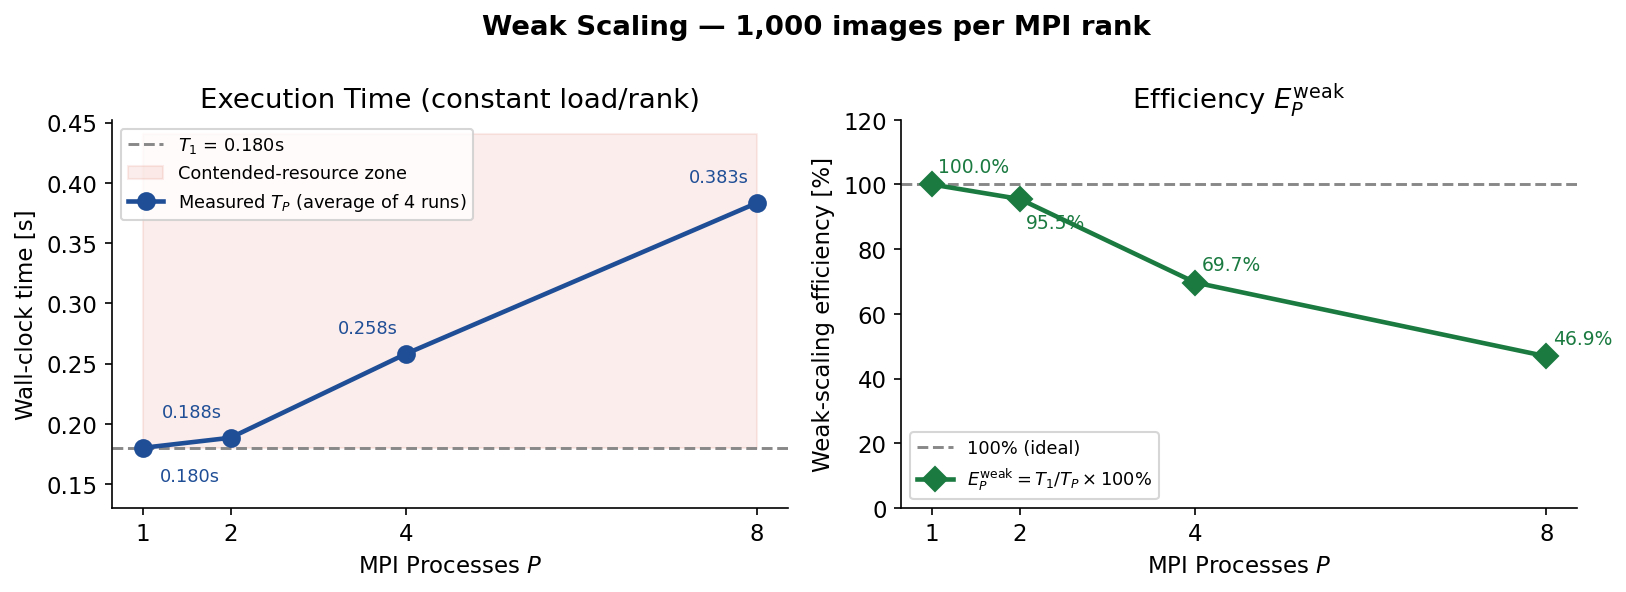
\includegraphics[width=0.85\textwidth]{weak_scaling.png}
\caption{Weak scaling: wall-clock time stays near $T_1$ through $P=2$, then grows
with $P$.}
\label{fig:weak-scaling}
\end{figure}

\needspace{3\baselineskip}
\section{GPU Concurrency Experiment}
\label{sec:gpu-scaling}


\subsection{Experimental Design}

The experiment (\texttt{experiments\slash{}run\_\discretionary{}{}{}gpu\_\discretionary{}{}{}scaling.py}, optionally with \texttt{-{}-reverse}) sweeps
$P \in \{1,2,4,8\}$ ranks, each processing 5{,}000 images, to quantify
how concurrent demand on the shared GPU affects throughput. Rank $r$
takes files $[5000r, 5000(r{+}1))$ of the file list, so both ranks
process JPEGs at $P=2$, while from $P=4$ later ranks receive the costlier
GeoTIFFs (Section~\ref{sec:stage-breakdown}): rank~2 holds 1{,}000 of them,
and rank~3 at $P=4$ and ranks 3--7 at $P=8$ hold only GeoTIFFs.

Each $P$ is measured across four sweeps, one in reverse rank order to expose drift,
with a coefficient of variation of 2--10\,\% (raw data:
\texttt{results\slash{}gpu\_\discretionary{}{}{}scaling\_\discretionary{}{}{}raw\_\discretionary{}{}{}sweeps.csv}).

\subsection{Results and Analysis}

Table~\ref{tab:gpu-scaling} and Figure~\ref{fig:gpu-concurrency} give the results.

\begin{table}[H]
\centering
\caption{GPU concurrency experiment: 5{,}000 images/rank, mean of 4
independent sweeps with 7\,GB held, all ranks sharing one integrated GPU.
Throughput is the mean over the sweeps; $T_P$ is total images divided by that
mean. The last column is a repeat without held memory (2 sweeps), with the
images cached.}
\label{tab:gpu-scaling}
\setlength{\tabcolsep}{4pt}
\begin{tabular}{@{}crrrcr@{}}
\toprule
$P$ & \textbf{Total images} & $T_P$ [s] &
\textbf{Throughput [img/s]} & $S_P^{\mathrm{thr}}$ & \textbf{Cached [img/s]} \\
\midrule
1 &  5,000 & 0.484 & 10,325 & 1.00$\times$ & 10,222 \\
2 & 10,000 & 0.685 & 14,606 & 1.41$\times$ & 17,677 \\
4 & 20,000 & 1.852 & 10,800 & 1.05$\times$ & 14,257 \\
8 & 40,000 & 4.712 &  8,489 & 0.82$\times$ & 18,860 \\
\bottomrule
\end{tabular}
\end{table}

\begin{figure}[H]
\centering
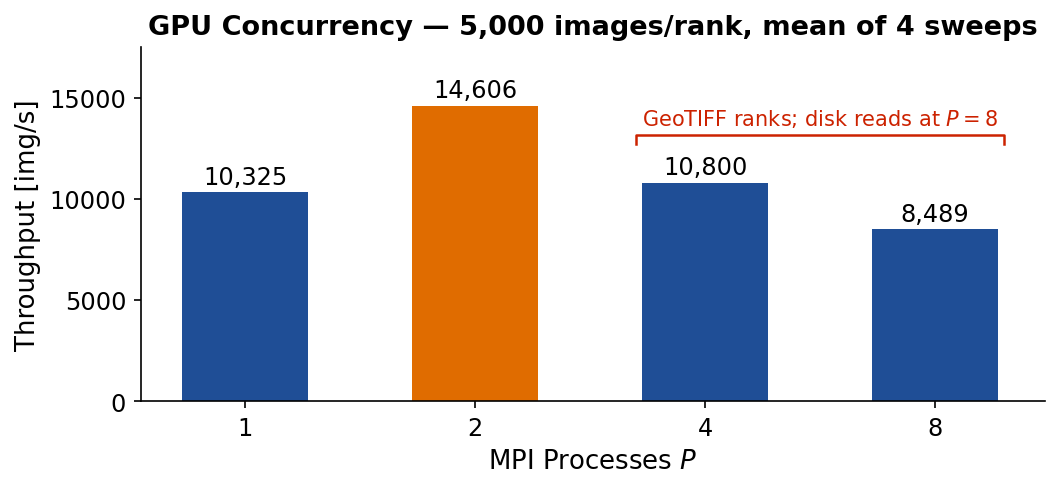
\includegraphics[width=0.65\textwidth]{gpu_concurrency.png}
\caption{GPU concurrency experiment: aggregate throughput peaks at
$P=2$, where both ranks process JPEGs, and falls from $P=4$, where GeoTIFF ranks
set the time and, at $P=8$, images are read from disk.}
\label{fig:gpu-concurrency}
\end{figure}

Throughput peaks at $P=2$ ($1.41\times$), where two JPEG ranks share the GPU with
contention for the device and the CPU cores. It falls at $P=4$ ($1.05\times$) and
$P=8$ ($0.82\times$) as per-rank times spread out: in the final run of the last
sweep they were 0.74--0.76\,s at $P=2$ ($T_2$ varied from 0.63\,s to 0.80\,s across
sweeps), 0.97--1.89\,s at $P=4$ and 1.45--4.34\,s at $P=8$. The pattern held in all
four sweeps. The repeat with the images cached shows how much of the fall is disk
access: throughput at $P=8$ is 18{,}860 images/s instead of 8{,}489, so that fall is
mainly reading from disk rather than GPU contention. The dip at $P=4$ remains, with
ranks spreading from 0.75\,s to 1.42\,s, which is the load imbalance of
Section~\ref{sec:stage-breakdown}. A multi-GPU node would remove the competition for
one device; this was not measured.

\subsection{Verification of GPU Utilisation}
\label{sec:gpu-idle-check}

\texttt{init\_\discretionary{}{}{}opencl()} requests
\texttt{CL\_\discretionary{}{}{}DEVICE\_\discretionary{}{}{}TYPE\_\discretionary{}{}{}GPU} and falls back to the CPU only if
no GPU is found; every run prints \texttt{[CPP] Rank~0 -> GPU[0]
Apple~M4}. An independent script using PyOpenCL
(\texttt{experiments\slash{}verify\_\discretionary{}{}{}gpu\_\discretionary{}{}{}profiling.py}), which reads
the production kernel source but bypasses the C++ library, confirms
non-zero driver-recorded device execution for all 214 batches. These
driver timestamps are used only as evidence of execution, not for
timing: they report about 0.03\,ms for a 64-image kernel run that the host
clock measures at about 2\,ms
(\texttt{experiments\slash{}verify\_\discretionary{}{}{}gpu\_\discretionary{}{}{}breakdown.py}), and only the
host clock grows with the batch size as the work does. That script's 2\,ms and
the 3.05\,ms in Table~\ref{tab:gpu-device-breakdown} differ through run-to-run
GPU state rather than method: alternating the two in one session gave
2.07--2.47\,ms and 1.73--4.29\,ms respectively.

\texttt{experiments\slash{}run\_\discretionary{}{}{}gpu\_\discretionary{}{}{}stage\_\discretionary{}{}{}timing.py} times the
production calls with the host clock, with \texttt{clFinish} after each
phase (25 trials per batch size after 5 discarded), and the same FFT on
the CPU.

\begin{table}[H]
\centering
\caption{Time per call [ms] of the GPU stages and of the same FFT on the
CPU, host clock, random $64\times64\times3$ images.}
\label{tab:gpu-device-breakdown}
\begin{tabular}{@{}rrrrrr@{}}
\toprule
\textbf{Batch} & \textbf{FFT kernel} & \textbf{FFT call} &
\textbf{Filter call} & \textbf{NumPy FFT} & \textbf{OpenMP FFT} \\
\midrule
16 & 1.78 & 2.31 & 0.76 & 1.53 & 0.81 \\
64 & 3.05 & 3.49 & 0.89 & 6.91 & 3.04 \\
256 & 4.91 & 5.61 & 2.14 & 25.39 & 11.65 \\
1024 & 17.13 & 18.78 & 7.46 & 103.08 & 44.61 \\
\bottomrule
\end{tabular}
\end{table}

Most of the FFT call is kernel execution, and the time grows with the batch.
A straight-line fit gives a fixed cost per FFT dispatch of about 2.0\,ms plus
16\,$\mu$s per image here, which is 36\,\% of the call at the production batch
of 256. Three repeats of the sweep gave a smaller fixed cost, 0.9--1.3\,ms
(16--23\,\% at 256), so this cost varies with GPU state, and the per-image cost
of 16--18\,$\mu$s is the stable figure. Larger batches amortise the fixed cost
(Section~\ref{sec:agglomeration}). At a batch of 256 the GPU FFT is about
$4.5\times$ faster than single-threaded NumPy and $2.1\times$ faster than the
ten-thread OpenMP path, and the call time reproduced within 4\,\% (5.6--5.8\,ms).
At a batch of 16 the OpenMP path is faster and NumPy comparable to the GPU. GPU
speed depends on its power state: in one earlier session the 256-image call took
15.5\,ms, slower than OpenMP (11.8\,ms) but still faster than NumPy (27.4\,ms).

Offloading is justified for this batch size,
but at $P=8$ the two GPU stages occupy only about 12\,\% of a
GeoTIFF rank's time (Table~\ref{tab:stage-breakdown}; 19\,\% in the repeat session), so a
multi-GPU deployment would relieve contention without removing the larger
limit, the Load stage.

\needspace{8\baselineskip}
\section{Additional Experiments}
\label{sec:additional-experiments}

\subsection{OpenMP Thread Scaling}

With a single MPI rank, \texttt{OMP\_\discretionary{}{}{}NUM\_\discretionary{}{}{}THREADS} is varied via
\texttt{experiments\slash{}run\_\discretionary{}{}{}openmp\_\discretionary{}{}{}scaling.py} while the whole single-rank
pipeline runs end to end on the first 20{,}000 files (14{,}000 JPEGs, 6{,}000
GeoTIFFs), in three interleaved rounds (Table~\ref{tab:openmp-scaling},
Figure~\ref{fig:openmp-scaling}).

\begin{table}[H]
\centering
\caption{OpenMP thread scaling ($P=1$, 20{,}000 images, mean of 3 interleaved
rounds).}
\label{tab:openmp-scaling}
\begin{tabular}{@{}crrr@{}}
\toprule
\textbf{Threads} & $T$ [s] & $S_t = T_1/T$ &
\textbf{Throughput [img/s]} \\
\midrule
1 & 2.131 & 1.00 & 9,384 \\
2 & 2.159 & 0.99 & 9,263 \\
4 & 2.141 & 1.00 & 9,343 \\
8 & 2.156 & 0.99 & 9,276 \\
\bottomrule
\end{tabular}
\end{table}

\begin{figure}[H]
\centering
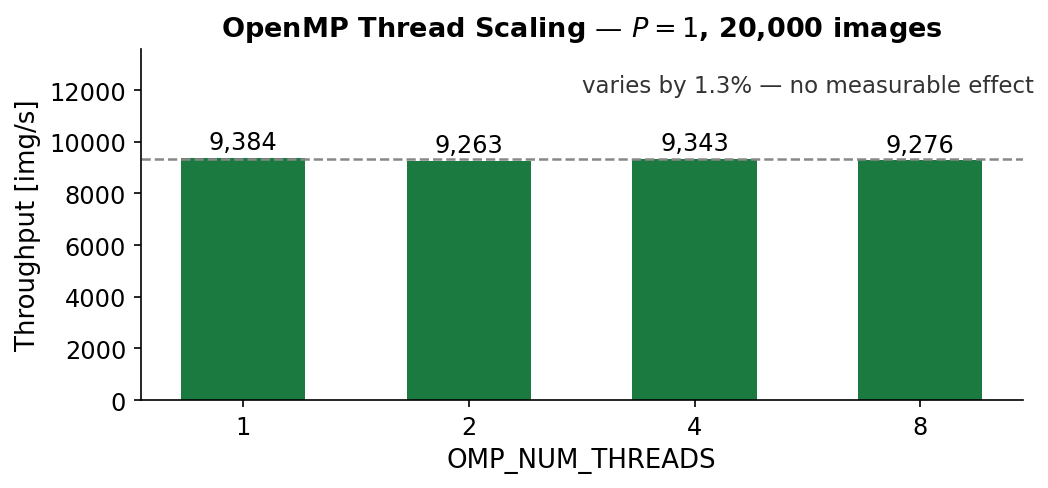
\includegraphics[width=0.65\textwidth]{openmp_scaling.png}
\caption{OpenMP thread scaling: throughput varies by less than 2\,\% across 1--8
threads.}
\label{fig:openmp-scaling}
\end{figure}

Thread count has no measurable effect on end-to-end pipeline time. This follows
from which code path runs: when a GPU is available, Stages~2--3 execute via the OpenCL kernels
rather than the OpenMP CPU-fallback paths
(\texttt{cpu\_\discretionary{}{}{}fft\_\discretionary{}{}{}magnitude}, \texttt{cpu\_\discretionary{}{}{}highpass}) also present
in \texttt{pipeline\_\discretionary{}{}{}kernels.cpp}. The \emph{only} OpenMP-parallel code
on the hot path is Stage~4's \texttt{extract\_\discretionary{}{}{}features\_\discretionary{}{}{}cpu}, which
was measured at 45\,ms on these 20{,}000 images -- about 2\,\% of the
$\approx$2.1\,s total, too small a share
for any thread count to produce a measurable effect. OpenMP
matters on a GPU-less deployment, where Stages~2--3 fall back to the CPU
paths above. Sweeping the OpenMP FFT path itself
(\texttt{experiments\slash{}run\_\discretionary{}{}{}openmp\_\discretionary{}{}{}fft\_\discretionary{}{}{}scaling.py}, 1{,}024 random
images, 5 interleaved rounds) gives 218.6, 112.0, 61.9, 46.9 and 43.4\,ms at
1, 2, 4, 8 and 10 threads: speedups of 1.95, 3.53, 4.67 and 5.03$\times$ (a repeat
reached $4.64\times$ at 10 threads), with the gain flattening beyond the 4
performance cores.

\subsection{Pipeline Stage Time Breakdown}
\label{sec:stage-breakdown}

\begin{table}[H]
\centering
\caption{Per-stage busy time at $P=8$ ($N=54{,}597$), measured by
timing the production stage functions under \texttt{mpirun -n 8}
(\texttt{experiments\slash{}run\_\discretionary{}{}{}stage\_\discretionary{}{}{}breakdown.py}),
average of 5 trials, for the JPEG ranks (0, 1, 7; 6{,}824--6{,}825 JPEGs
each) and the GeoTIFF ranks (3, 4, 5; 6{,}824--6{,}825 GeoTIFFs each);
ranks 2 and 6 hold a mix. Stages overlap in
the pipeline, so busy times do not add up to the wall time.}
\label{tab:stage-breakdown}
\begin{tabular}{@{}lrrc@{}}
\toprule
\textbf{Stage} & \textbf{JPEG rank [s]} & \textbf{GeoTIFF rank [s]} &
\textbf{Device} \\
\midrule
$S_1$: Load \& Preprocess & 2.41 & \textbf{5.65} & CPU \\
$S_2$: FFT magnitude      & 0.44 & 0.52 & GPU (OpenCL) \\
$S_3$: High-pass filter   & 0.19 & 0.20 & GPU (OpenCL) \\
$S_4$: Feature extraction & 0.04 & 0.05 & CPU (OpenMP) \\
\midrule
\textbf{Rank wall time}   & 2.56 & \textbf{5.79} & \\
\bottomrule
\end{tabular}
\end{table}

The ranks hold the same number of images, yet the GeoTIFF ranks take
more than twice as long, and almost the whole difference lies in the Load
stage: a 13-band GeoTIFF is about
31$\times$ larger on disk than a JPEG and is decoded with
\texttt{tifffile} rather than Pillow, while the GPU and feature stages
cost nearly the same for both. The slowest rank is a GeoTIFF rank in every
trial, and on the GeoTIFF ranks Load is busy for 98\,\% of the wall time (GPU
stages 9\,\% and 3\,\%, features 1\,\%), so Load is the bottleneck stage.
Replacing the contiguous split by a cyclic one
(\texttt{all\_files[rank::size]}), which gives every rank the same
JPEG/GeoTIFF mix, was measured with the production pipeline patched from
outside (\texttt{experiments\slash{}run\_\discretionary{}{}{}partition\_\discretionary{}{}{}comparison.py}, 3
alternating trials, Table~\ref{tab:partition}): it reduced $T_P$ by 35\,\% at
$P=4$ and 28\,\% at $P=8$ ($-38\,\%$ and $-35\,\%$ in the repeat session), and in
all six cyclic runs the fastest and slowest ranks finished within 0.13\,s of each
other. The contiguous times differ from Table~\ref{tab:strong-scaling}, measured in
a separate session (Section~\ref{sec:methodology}). $P=2$ was not measured, since
its ranks are already close.

\begin{table}[H]
\centering
\caption{Contiguous versus cyclic partition, mean of 3 alternating trials
(\texttt{results\slash{}partition\_\discretionary{}{}{}comparison.csv}). The first column repeats
Table~\ref{tab:strong-scaling} (a separate session) for reference.}
\label{tab:partition}
\begin{tabular}{@{}crrrr@{}}
\toprule
$P$ & \textbf{Table~\ref{tab:strong-scaling} [s]} & \textbf{Contiguous [s]} &
\textbf{Cyclic [s]} & \textbf{Change} \\
\midrule
4 & 7.06 & 7.91 & 5.14 & $-35\,\%$ \\
8 & 5.37 & 5.70 & 4.10 & $-28\,\%$ \\
\bottomrule
\end{tabular}
\end{table}

The contiguous split remains the production design because the cyclic split was
measured after all other experiments, which use the contiguous split; changing it
would have broken their comparability. Adopting the cyclic split is the first item of
future work.

\subsection{Pipeline Stage-Overlap Verification}
\label{sec:pipeline-overlap-verification}

Table~\ref{tab:pipeline-timing} presents measured per-batch
stage start/end times recorded by
\texttt{experiments\slash{}run\_\discretionary{}{}{}pipeline\_\discretionary{}{}{}timing.py} in pipeline mode
(512 images, batch size 64, single rank).
Batch~1 Load (4.14--8.43\,ms) overlaps with Batch~0 GPU execution
(4.15--7.11\,ms) for their entire common window, and Batch~0 CPU
(7.13--7.38\,ms) falls inside the still-running Batch~1 Load interval.
The table is one representative run; stage times vary (Batch~0 GPU took 5.3\,ms
in a repeat), but the script's \texttt{[VERIFIED] Pipeline overlap} line confirmed the
Load/GPU overlap in every run. The GPU stage here (2.96\,ms) is
shorter than the 4.38\,ms of Table~\ref{tab:gpu-device-breakdown} at the same batch size
(3.49 + 0.89\,ms): a different session, within the range of GPU-state variation
(1.73--4.29\,ms, Section~\ref{sec:gpu-idle-check}).

\begin{table}[H]
\centering
\caption{Measured pipeline timing ($P=1$, batch size 64,
relative wall-clock milliseconds).}
\label{tab:pipeline-timing}
\setlength{\tabcolsep}{4pt}
\begin{tabular}{@{}ccrrrc@{}}
\toprule
\textbf{Batch} & \textbf{Stage} &
\textbf{Start [ms]} & \textbf{End [ms]} & \textbf{Duration [ms]} &
\textbf{Overlap?} \\
\midrule
0 & Load  & 0.06 & 4.14 & 4.08 & --- \\
0 & GPU   & 4.15 & 7.11 & 2.96 & --- \\
1 & Load  & 4.14 & 8.43 & 4.29 &
  \textcolor{TealCPU!70!black}{\textbf{Yes (with Batch 0 GPU)}} \\
0 & CPU   & 7.13 & 7.38 & 0.26 &
  \textcolor{TealCPU!70!black}{\textbf{Yes (with Batch 1 Load)}} \\
1 & GPU   & 8.44 & 11.54 & 3.10 &
  \textcolor{TealCPU!70!black}{\textbf{Yes (with Batch 2 Load)}} \\
2 & Load  & 8.44 & 12.73 & 4.29 &
  \textcolor{TealCPU!70!black}{\textbf{Yes (with Batch 1 GPU)}} \\
\bottomrule
\end{tabular}
\end{table}

\subsection{Task-Parallelism Payoff: Pipeline Mode vs.\ Sequential Mode}
\label{sec:pipeline-payoff}

Pipeline mode is compared end to end with sequential mode
(Section~\ref{sec:prefetch-task-parallelism}) on the full dataset at $P=1$ and $P=8$. Three rounds alternate the two
modes, each timed run preceded by an untimed run of the same mode, without held
memory (\texttt{experiments\slash{}run\_\discretionary{}{}{}pipeline\_\discretionary{}{}{}onoff\_\discretionary{}{}{}comparison.py}).

\begin{table}[H]
\centering
\caption{Pipeline mode versus sequential mode, full dataset, mean of 3
alternating rounds.}
\label{tab:pipeline-onoff}
\begin{tabular}{@{}crrr@{}}
\toprule
$P$ & \textbf{Pipeline ON [s]} & \textbf{Pipeline OFF [s]} &
\textbf{Speedup} \\
\midrule
1 & 6.32 & 22.04 & $3.49\times$ \\
8 & 2.59 & 5.99 & $2.32\times$ \\
\bottomrule
\end{tabular}
\end{table}

Pipeline mode is faster than sequential mode in every one of the
twelve timed runs; a repeat of the experiment gave $3.37\times$ and $2.51\times$.
Two mechanisms contribute.
The first is stage overlap: overlap alone bounds the
speedup of a pipeline limited by its slowest stage at
$(t_{\mathrm{load}}+t_{\mathrm{gpu}}+t_{\mathrm{cpu}})
/\max(t_{\mathrm{load}},t_{\mathrm{gpu}},t_{\mathrm{cpu}})$, which is about
$1.8\times$ with the stage times of Table~\ref{tab:pipeline-timing} and $1.9\times$
in the repeat of that measurement.
The second is the file cache: sequential mode materialises the rank's
entire subset and its spectrum and filtered copies (about 5\,GB resident
at $P=1$), against an estimated bound of $\approx$240\,MB per rank for the pipeline
(Section~\ref{sec:agglomeration}). This footprint evicts the images
from the OS file cache, so sequential runs read them from disk while pipeline
runs keep them cached. Starting from a cached state at $P=1$, a sequential run took 11.0\,s against
6.3\,s for pipeline runs ($1.75\times$, close to the overlap bound), and
the pipeline run directly after it took 17.4\,s before returning to
6.3\,s. Table~\ref{tab:pipeline-onoff} shows each mode's steady state.

\section{Summary and Comparative Benchmarking}
\label{sec:comparative-benchmarking}

The sequential row is a single-threaded, pure NumPy implementation of
Algorithm~\ref{alg:seq} (no MPI, OpenMP or OpenCL) with the project's own loader,
timed in the same three rounds as the hybrid runs
(\texttt{experiments\slash{}run\_\discretionary{}{}{}comparative\_\discretionary{}{}{}benchmark.py}), and
the hybrid pipeline was faster in every round (Table~\ref{tab:comparative},
Figure~\ref{fig:comparative-benchmark}). All rows compute the same result: the
sequential program and the pipeline agree to within $10^{-6}$ on 3{,}000 random
files, and the pipeline with NumPy on all files (Chapter~\ref{chap:rationale}).

\begin{table}[H]
\centering
\caption{Comparative performance for $N=54{,}597$ images: mean of 3
rounds in which all five implementations are timed
(\texttt{results\slash{}comparative\_\discretionary{}{}{}benchmark.csv}).}
\begin{tabular}{@{}lrr@{}}
\toprule
\textbf{Implementation} & $T$ [s] & \textbf{Speedup vs.\ sequential} \\
\midrule
Sequential (1 thread, pure NumPy, no MPI/GPU) & 22.61 & 1.00$\times$ \\
Hybrid pipeline, $P=1$ & 15.86 & 1.43$\times$ \\
Hybrid pipeline, $P=2$ & 9.45 & 2.39$\times$ \\
Hybrid pipeline, $P=4$ & 6.95 & 3.25$\times$ \\
\textbf{Hybrid pipeline, $P=8$} & \textbf{5.04} &
  \textbf{4.49}$\times$ \\
\bottomrule
\end{tabular}
\label{tab:comparative}
\end{table}

\begin{figure}[H]
\centering
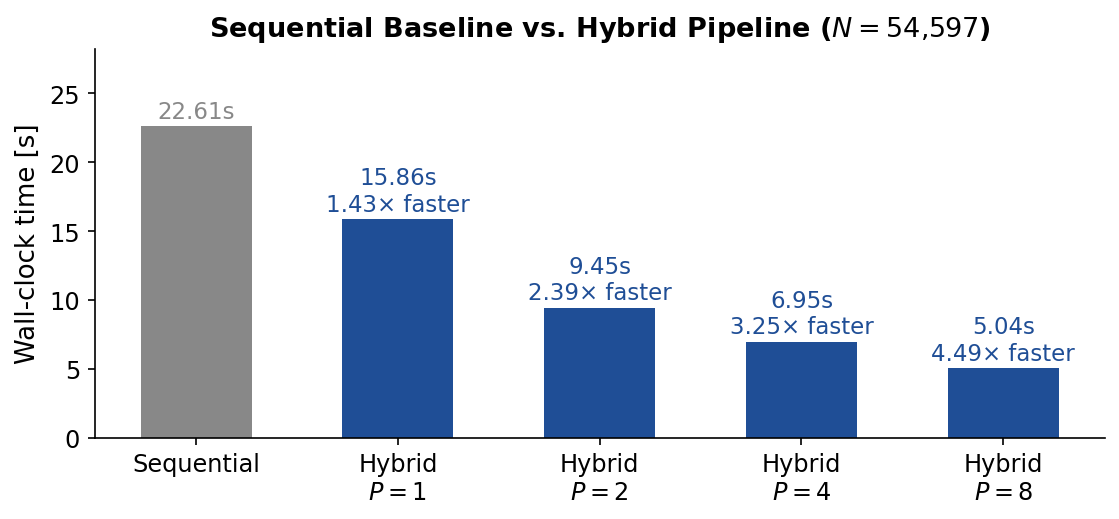
\includegraphics[width=0.62\textwidth]{comparative_benchmark.png}
\caption{Sequential baseline versus the hybrid pipeline at each $P$. The hybrid
pipeline is faster at every $P$, including $P=1$.}
\label{fig:comparative-benchmark}
\end{figure}

At $P=1$ the hybrid pipeline is already $1.43\times$ faster: the sequential loop
spends 69.8\,\% of its time loading and 26.2\,\% in the FFT, whereas in the
pipeline Stages~2--4 overlap with loading, so the $P=1$ time is essentially the
Load stage alone (about 15.7\,s of the sequential run, against 15.86\,s). MPI
raises the advantage to $4.49\times$ at $P=8$, limited by the load imbalance
(Section~\ref{sec:stage-breakdown}); with the images cached the times are 13.5\,s
sequential and 6.80\,s and 2.64\,s at $P=1$ and $P=8$ ($1.98\times$ and $5.11\times$).

%=======================================================================
\chapter{Conclusions}
\label{chap:conclusions}
%=======================================================================

\section{Summary}

This project designed, implemented, and evaluated a hybrid MPI + OpenCL + OpenMP
pipeline for frequency-domain processing of 54{,}597 EuroSAT image files, combining
data parallelism across ranks, task parallelism within each rank, and a
configurable workflow with minimal communication.

\paragraph{Principal findings.}
The pipeline reaches $\approx$10{,}200 images/s at $P=8$
($S_8 \approx 3.17$, and 2.2--3.2 across repeat sessions; efficiency 92.9\,\% at $P=2$), $1.43\times$/$4.49\times$
faster than the sequential baseline at $P=1$/$P=8$, with features matching
a NumPy reference; pipelined execution is $2.3\times$ faster than
sequential-stage execution at $P=8$, with stage overlap explaining at most
about $1.9\times$ and a file-cache effect the rest. Scaling is limited mainly by load imbalance from $P=4$
(mainly-JPEG versus mainly-GeoTIFF ranks) and secondarily by the shared
GPU; the Load stage, not the GPU, is the bottleneck. OpenMP has no measurable
end-to-end effect while the GPU runs Stages~2--3, because the only OpenMP stage on
that path takes about 2\,\% of the time, but on the CPU FFT path used without a GPU
it gives about $5\times$ at 10 threads.

\section{Limitations and Future Work}
\label{sec:limitations}\label{sec:future-work}

\begin{itemize}[noitemsep]
  \item \textbf{Load imbalance.} A cyclic split gives every rank the
    same JPEG/GeoTIFF mix; it reduced $T_8$ by 28\,\% when measured.
  \item \textbf{Single node, one GPU.} Multi-node scaling is unmeasured.
  \item \textbf{FFT kernel.} It handles power-of-two sizes in single
    precision; batched libraries such as clFFT \cite{amd2014} offer more.
  \item \textbf{GPU dispatch cost.} Persistent buffers could reduce the fixed cost
    per dispatch.
  \item \textbf{Laptop testbed.} Timings and speedups depend on the OS file
    cache, which is only partly controlled here.
\end{itemize}

%=======================================================================
\renewcommand{\bibname}{References}
\begin{singlespace}
\begin{thebibliography}{99}
\addcontentsline{toc}{chapter}{References}
\setlength{\itemsep}{0pt}

\bibitem{amd2014}
AMD (2014).
\textit{clFFT: OpenCL Fast Fourier Transform Library}.
AMD Open Source. \url{https://github.com/clMathLibraries/clFFT}

\bibitem{amdahl1967}
Amdahl, G.~M. (1967).
Validity of the single processor approach to achieving large scale
computing capabilities.
In \textit{Proceedings of the AFIPS Spring Joint Computer Conference},
pages 483--485.

\bibitem{applem4}
Apple (2025). \textit{MacBook Air (13-inch, M4, 2025) -- Tech Specs}.
\url{https://support.apple.com/en-us/122209}

\bibitem{cooley1965}
Cooley, J.~W. and Tukey, J.~W. (1965).
An algorithm for the machine calculation of complex Fourier series.
\textit{Mathematics of Computation}, 19(90):297--301.

\bibitem{drusch2012}
Drusch, M. et al. (2012).
Sentinel-2: ESA's optical high-resolution mission for GMES operational
services.
\textit{Remote Sensing of Environment}, 120:25--36.

\bibitem{foster1995}
Foster, I. (1995). \textit{Designing and Building Parallel Programs}.
Addison-Wesley.

\bibitem{frigo2005}
Frigo, M. and Johnson, S.~G. (2005).
The design and implementation of FFTW3.
\textit{Proceedings of the IEEE}, 93(2):216--231.

\bibitem{fftwmpi}
Frigo, M. and Johnson, S.~G. \textit{FFTW 3 Manual: Distributed-memory FFTW
with MPI}. \url{https://www.fftw.org/fftw3_doc/Distributed_002dmemory-FFTW-with-MPI.html}

\bibitem{gorelick2017}
Gorelick, N. et al. (2017).
Google Earth Engine: Planetary-scale geospatial analysis for everyone.
\textit{Remote Sensing of Environment}, 202:18--27.

\bibitem{helber2019}
Helber, P. et al. (2019).
EuroSAT: A novel dataset and deep learning benchmark for land use
and land cover classification.
\textit{IEEE Journal of Selected Topics in Applied Earth Observations
and Remote Sensing}, 12(7):2217--2226.

\bibitem{karp1990}
Karp, A.~H. and Flatt, H.~P. (1990).
Measuring parallel processor performance.
\textit{Communications of the ACM}, 33(5):539--543.

\bibitem{mpiforum2021}
MPI Forum (2021).
\textit{MPI: A Message-Passing Interface Standard, Version 4.0}.
Technical report. \url{https://www.mpi-forum.org/docs/mpi-4.0/mpi40-report.pdf}

\bibitem{openmpARB2018}
OpenMP Architecture Review Board (2018).
\textit{OpenMP Application Programming Interface, Version 5.0}.
\url{https://www.openmp.org/specifications/}

\bibitem{rauber2013}
Rauber, T. and R\"{u}nger, G. (2013).
\textit{Parallel Programming: For Multicore and Cluster Systems}.
2nd edition. Springer, Berlin.

\bibitem{stone2010}
Stone, J.~E., Gohara, D., and Shi, G. (2010).
OpenCL: A parallel programming standard for heterogeneous computing
systems.
\textit{Computing in Science \& Engineering}, 12(3):66--73.

\end{thebibliography}
\end{singlespace}

\end{document}
